%% abtex2-modelo-slides.tex, v-1.0 gfabinhomat
%% Copyright 2012-2014 by abnTeX2 group at http://abntex2.googlecode.com/ 
%%
%% This work may be distributed and/or modified under the
%% conditions of the LaTeX Project Public License, either version 1.3
%% of this license or (at your option) any later version.
%% The latest version of this license is in
%%   http://www.latex-project.org/lppl.txt
%% and version 1.3 or later is part of all distributions of LaTeX
%% version 2005/12/01 or later.
%%
%% This work has the LPPL maintenance status `maintained'.
%% 
%% The Current Maintainer of this work is Fábio Rodrigues Silva, 
%% member of abnTeX2 team, led by Lauro César Araujo. 
%% Further information are available on 
%% http://abntex2.googlecode.com/
%%
%% This work consists of the files abntex2-modelo-slides.tex, 
%% abntex2-modelo-references.bib and abntex2-modelo-marca.pdf
%%
%% Modelo desenvolvido por Fábio Rodrigues Silva (gfabinhomat@gmail.com)
%% Mais informações podem ser obtidas no guia do usuário Beamer 
%% (http://linorg.usp.br/CTAN/macros/latex/contrib/beamer/doc/beameruserguide.pdf)
%% Informações rápidas podem ser acessadas em http://en.wikibooks.org/wiki/LaTeX/Presentations


% Apresentações em widescreen. Outros valores possíveis: 1610, 149, 54, 43 e 32.
% Por padrão, as apresentações são no formato 4:3 (sem o aspectratio).
\documentclass[aspectratio=169]{beamer}	 	

\titulo{Improvisações de códigos para análise de um algoritmo tonal no \emph{A Study in Keith} (2009) de Andrew Sorensen}
\autor{Guilherme Martins Lunhani}

\instituicao{Universidade Federal de Juiz De Fora -- UFJF
  \par
  Instituto de Artes e Design -- IAD
  \par
  Programa de Pós-Graduação em Artes Visuais, Música e Tecnologia}

\orientador[Orientador: ]{Prof. Dr. Luiz Eduardo Castelões}

\data{\today}

% \changes{Versão inicial }{2013/07/22 }{v0.0.3}
\tipotrabalho{Tese (Mestrado)}

% O preambulo deve conter o tipo do trabalho, o objetivo, 
% o nome da instituição e a área de concentração 
\preambulo{Dissertação corrigida para a banca de qualificação no Programa Mestrado em Artes, Cultura e Linguagens do Instituto de Artes e Design da Universidade Federal de Juiz de Fora (UFJF), linha de Artes Visuais, Musica e Tecnologia.}
%\EnableCrossrefs
%\CodelineIndex
%\RecordChanges

% ---
% Configurações de aparência do PDF final

% alterando o aspecto da cor azul
\definecolor{blue}{RGB}{41,5,195}

% informações do PDF
\makeatletter
\hypersetup{
     	%pagebackref=true,
		pdftitle={\@title}, 
		pdfauthor={\@author},
    	pdfsubject={\imprimirpreambulo},
	    pdfcreator={LaTeX with abnTeX2},
		pdfkeywords={abnt}{latex}{abntex}{abntex2}{trabalho acadêmico}, 
		colorlinks=true,       		% false: boxed links; true: colored links
    	linkcolor=blue,          	% color of internal links
    	citecolor=blue,        		% color of links to bibliography
    	filecolor=magenta,      		% color of file links
		urlcolor=blue,
		bookmarksdepth=4
}
\makeatother

%\newcommand{\todosautoresdelivecoding}{\begin{inparaenum}[]\item \citeonline{collins_live_2003},\item \citeonline{collins_generative_2003},\item \citeonline{collins_live_2003-1},\item \citeonline{wang_--fly_2004},\item \citeonline{ward_live_2004},\item \citeonline{blackwell_programming_2005},\item \citeonline{collins_live_2007},\item \citeonline{griffiths_fluxus:_2008},\item \citeonline{mclean_patterns_2009},\item \citeonline{rohrhuber_improvising_2009},\item \citeonline{mclean_visualisation_2010},\item \citeonline{magnusson_algorithms_2011},\item \citeonline{mccallum_show_2011},\item \citeonline{magnusson_herding_2014},\item \citeonline{magnusson_scoring_2014},\item \citeonline{collins_algorave:_2014},\item \citeonline{sorensen_livecodings_2014}\end{inparaenum}}
% --- 
% Espaçamentos entre linhas e parágrafos 
% --- 

% O tamanho do parágrafo é dado por:
\setlength{\parindent}{1.3cm}

% Controle do espaçamento entre um parágrafo e outro:
\setlength{\parskip}{0.2cm}  % tente também \onelineskip

% ---
% compila o indice
% ---
\makeindex

% ---
% Pacotes básicos 
% ---
\usepackage[utf8]{inputenc}		% Codificacao do documento (conversão automática dos acentos)
\usepackage{lmodern}			% Usa a fonte Latin Modern			
\usepackage[T1]{fontenc}		% Selecao de codigos de fonte.
\usepackage{lastpage}			% Usado pela Ficha catalográfica
\usepackage{indentfirst}		% Indenta o primeiro parágrafo de cada seção.
\usepackage{color}				% Controle das cores
\usepackage{graphicx}			% Inclusão de gráficos
\usepackage{wallpaper}			% inclusao de imagens deslocadas
\usepackage{microtype} 			% para melhorias de justificação
\usepackage{url}
\usepackage[table,xcdraw]{xcolor}
\usepackage{tabularx}
\usepackage{minted}
\usepackage{amsmath,amssymb}
\usepackage{framed}
\usepackage[amsmath,framed]{ntheorem}
\usepackage{pdfpages}

% ---
		
% ---
% Pacotes adicionais, usados apenas no âmbito do Modelo Canônico do abnteX2
% ---
\usepackage{lipsum}				% para geração de dummy text
% ---

%---
% Pacote para listas em uma linha
%---
\usepackage{paralist}

% ---
% Epigrade
% ---
\usepackage{epigraph}

% Front end para amsthm (\declaretheorem)
\usepackage{thmtools}    

% ---
% Pacotes de citações
% ---
\usepackage[brazilian,hyperpageref]{backref}	 % Paginas com as citações na bibl
\usepackage[alf]{abntex2cite}	% Citações padrão ABNT

%TODO
\usepackage[colorinlistoftodos]{todonotes}
%\usepackage{ntheorem}

\usepackage{tablefootnote}


%%%%%%%%%%% syntax highlight %%%%%%%%%%%%%%%%%%%%%%%%%%%%%%%%%%%%%%%%%%%%%%%%%%%%%
\usepackage{listings}
\definecolor{maroon}{rgb}{0.5,0,0}
\definecolor{darkgreen}{rgb}{0,0.5,0}
\definecolor{deepblue}{rgb}{0,0,0.5}
\definecolor{deepred}{rgb}{0.6,0,0}
\definecolor{purple}{rgb}{0.5,0,0.5}
\definecolor{deepgreen}{rgb}{0,0.5,0}
%%%%%%%%%%%%%%%%%%%%%%%%%%%%%%%%%%%%%%%%%%%%%%%%%%%%%%% 

\usepackage{tikz}
\tikzset{
  treenode/.style = {shape=rectangle, rounded corners,
                     draw, align=center,
                     top color=white, bottom color=blue!20},
  root/.style     = {treenode, font=\Large, bottom color=red!30},
  env/.style      = {treenode, font=\ttfamily\normalsize},
  dummy/.style    = {circle,draw}
}


% ----------------- INÍCIO DO DOCUMENTO --------------------------------------
\begin{document}

% ----------------- NOVO SLIDE --------------------------------
\input{./titulo}

% ----------------- NOVO SLIDE --------------------------------
\begin{frame}{Sumário}
\tableofcontents
\end{frame}

% ----------------- NOVO SLIDE --------------------------------
\section{Preambulo}
\begin{frame}{Preâmbulo}
O tema da improvisação de códigos, como um universo de conceitos, surgiu de uma experiência com um código em linguagem \emph{python} (\url{https://www.python.org}), útil para gerar um mapa de termos, como ilustrado na figura abaixo.
\end{frame}

% ----------------- NOVO SLIDE --------------------------------
\begin{frame}{Preâmbulo}
\begin{figure}
\centering
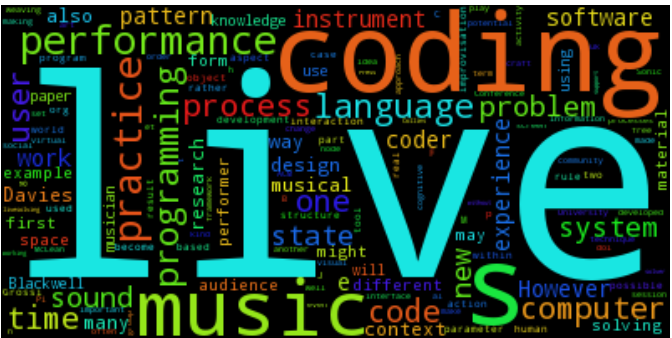
\includegraphics[scale=0.8]{imagens/nuvem.png}
\caption{Nuvem de palavras do \citeonline{ICLC2015},  1$^o$ Congresso Internacional de Live Coding. \textbf{Fonte}: autor.}
\label{fig:nuvemlivecoding}
\end{figure}
\end{frame}

\section{Introdução}
% ----------------- NOVO SLIDE --------------------------------
\begin{frame}{Introdução}
Metáfora:

Livecoding como venda de filosofias $\rightarrow$ Mercado emergente do conhecimento das artes computacionais.
\end{frame}

% ----------------- NOVO SLIDE --------------------------------
\begin{frame}{Introdução}
Metáfora:

Livecoding (improvisação de códigos) como venda de filosofias $\rightarrow$ Mercado emergente do conhecimento das artes computacionais.
\end{frame}

% ----------------- NOVO SLIDE --------------------------------
\begin{frame}{Introdução}
Abordagem do conhecimento das artes computacionais no \emph{Livecoding}:

• Conhecimento ortopédico $\rightarrow$ Universo de conceitos, bricolagem

• Razão indolente $\rightarrow$ metáforas e imagens mentais de uma improvisação de códigos são reduzidos como um objeto com diversas propriedades.

• Pensamento abissal $\rightarrow$ divisão dos que praticam o \emph{Livecoding} do ambiente europeu, e dos que não praticam fora do contexto europeu.
\end{frame}

% ----------------- NOVO SLIDE --------------------------------
\begin{frame}{Introdução}
Abordagem do conhecimento das artes computacionais no \emph{Livecoding}:
• Universo de conceitos
\end{frame}

\begin{frame}{Objetivo}
• Investigar um Universo de Conceitos sobre a \emph{improvisação de códigos} (\emph{live coding});

• Investigar um Espaço de Conceitos, historicamente restrito, sobre a improvisação de códigos;

• Investigar um método de análise/criação para uma improvisação de códigos;

• Investigar um Espaço Conceitual de uma improvisação de códigos, \emph{A Study in Keith} (2009) de Andrew Sorensen, e seu algoritmo musical em um ciclo de transformação.
\end{frame}

\section{Definições de base da Improvisação de códigos}
% ----------------- NOVO SLIDE --------------------------------
\begin{frame}{Definições de base da Improvisação de códigos}
\emph{Live coding} é uma técnica artística de improvisação. Pode ser empregada em muitos contextos diferentes de performance: dança, música, imagens em movimento e mesmo tecelagem. Eu concentrei minha atenção no lado musical, que parece ser o mais proeminente \cite[p.~117]{mori_analysing_2015}
\end{frame}

% ----------------- NOVO SLIDE --------------------------------
\begin{frame}{Definições de base da Improvisação de códigos}
A definição denota a aplicação em qualquer outra área, não apenas como metáfora, mas como estratégia de gerenciamento de fluxos criativos, assistidos por computador
\end{frame}

% ----------------- NOVO SLIDE --------------------------------
\begin{frame}{Tecelagem}
O grupo \emph{Weaving codes} foi formado para  a \emph{(\ldots) investigação de padrões a partir das perspectivas de tecelagem e música, e através do desenvolvimento de uma linguagem de computador e código para descrever a construção de tecidos} \cite{griffths_weave_2015}
\end{frame}

% ----------------- NOVO SLIDE --------------------------------
\begin{frame}{Tecelagem}
\emph{Uma das idéias originais era combinar tecelagem e codificação em um cenário de atuação, ambos para fornecer uma forma de tornar a codificação ao vivo mais inclusiva com a tecelagem, e ao mesmo tempo esclarecer os processos de pensamentos digitais envolvolvidos na tecelagem (\ldots) Nossa audiência consistiu de pesquisadores de artesanato, biólogos antropológicos, arquitetos, designers de jogos e tecnólogos -- foi mais do que antecipamos! Alex e eu disponibilizamos alguns códigos de música do \emph{slub} para tecer, e minha parte favorita foi projetar a tecelagem ao vivo} \cite{griffths_weave_2015}.
\end{frame}

% ----------------- NOVO SLIDE --------------------------------
\defverbatim[colored]{\tecelagem}{
\begin{minted}[fontsize=\scriptsize]{cl}
(twist 3 4 5 14 15 16)
(weave-forward 3)
(twist 4 15)
(weave-forward 1)
(twist 4 8 11 15)

(repeat 2
 (weave-back 4)
 (twist 8 11)
 (weave-forward 2)
 (twist 9 10)
 (weave-forward 2)
 (twist 9 10)
 (weave-back 2)
 (twist 9 10)
 (weave-back 2)
 (twist 8 11)
 (weave-forward 4))
\end{minted}
}

\begin{frame}{Tecelagem}
\tecelagem
\end{frame}

% ----------------- NOVO SLIDE --------------------------------
\begin{frame}{Tecelagem}
\begin{figure}[!h]
    \centering
    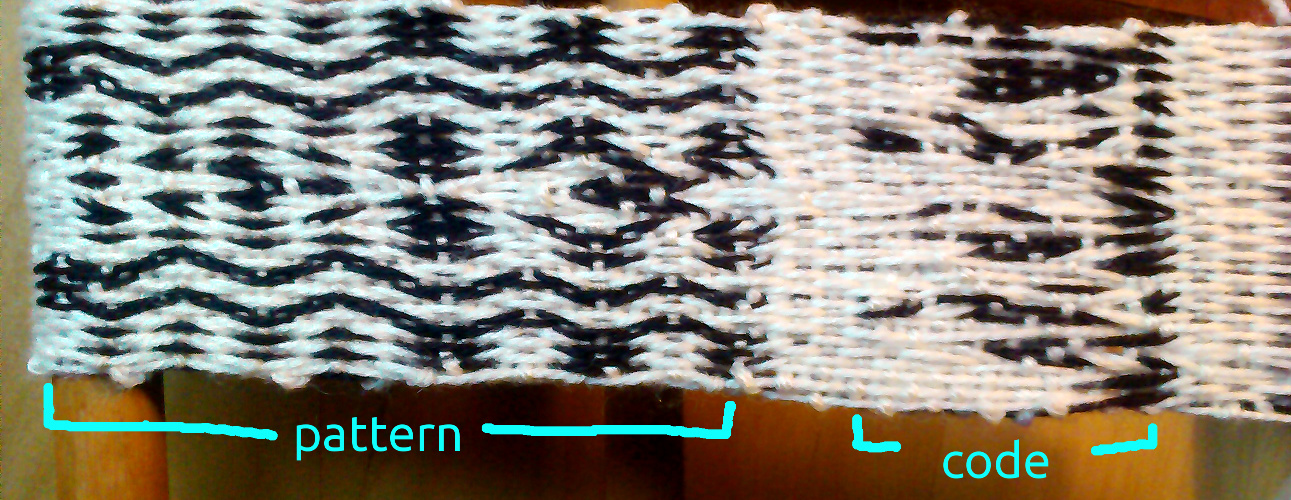
\includegraphics[scale=0.31]{imagens/weaving.jpg}
    \caption{Tecido resultante da prática \emph{Weaving code}. \textbf{Fonte}: \citeonline{griffths_weave2_2015}.}
  \label{fig:weaving}
\end{figure}
\end{frame}

% ----------------- NOVO SLIDE --------------------------------
\begin{frame}{Tecelagem}
• Apresentação de dois importantes personagens para o \emph{Livecoding}: Alex McLean e Dave Griffths (\emph{Slub})

• Observação de possíveis rituais de \emph{livecoding}, como apresentação artística informal/formal.
\end{frame}

% ----------------- NOVO SLIDE --------------------------------
\begin{frame}{Tecelagem}
\begin{figure}[h]
  \centering
  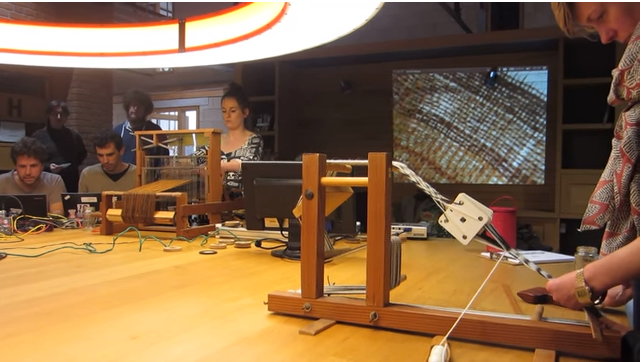
\includegraphics[scale=0.5]{imagens/weaving.png}
  \caption{Performance no Foam Kernow. \textbf{Fonte}: \citeonline{griffths_weave_2015}.}
  \label{fig:weavecoding}
\end{figure}
\end{frame}

% ----------------- NOVO SLIDE --------------------------------
\begin{frame}{Slub}
A banda \emph{Slub} começou em 2000, como uma colaboração entre Adrian Ward e Alex McLean. A premissa do duo era utilizar a atividade de programação para realização de uma Música Eletrônica de Dança\footnote{\cfcite{hillegonda_dj_2013}}. Sua primeira reunião foi em 2001, no \emph{Paradiso club} em Amsterdã, durante o festival \emph{Sonic Arts}. Em 2005 Griffths se juntou ao duo durante o festival \emph{Sonar}, o que abriu espaço para o desenvolvimento de uma estética de videogames \cite[p.~138--140]{McLean2011}.
\end{frame}

% ----------------- NOVO SLIDE --------------------------------
\begin{frame}{Live coding como dança}
• Dança como fim de uma improvisação de códigos $\rightarrow$ Algorave 

• Dança como meio (coreografia) de uma improvisação de códigos $\rightarrow$ Kate Sichio 
\end{frame}

% ----------------- NOVO SLIDE --------------------------------
\begin{frame}{Algorave}
\emph{\emph{Algorave} 'comecou como uma piada', de acordo com Alex McLean, um pesquisador de música computacional e um dos três de uma banda chamada \emph{Slub}, que têm improvisado códigos por 13 anos. Ele veio com um termo enquanto conduzia uma \emph{gig} em Nottingham com seu amigo Nick Collins (que tocava ``datapop'' sob o nome Sick Lincoln) no final de 2011. 'Nós sintonizamos em uma estação pirata tocando \emph{happy hardcore}, e nós pensamos que seria bom programar alguma música \emph{rave}.' Deste então, McLean organizou oito \emph{algoraves} informais no mundo.} \cite{chesire_algorave_2013}
\end{frame}

% ----------------- NOVO SLIDE --------------------------------
\begin{frame}{Algorave}
\emph{\emph{Algorave} não é sustentado exclusivamente por \emph{live coders}, mas estes têm mantido uma forte presença em todos os eventos até agora. É assim talvez porque a tradição do \emph{live coding} de projetar telas motiva todo o esforço; onde algoritmos não estão visíveis por períodos de tempo durante uma \emph{algorave}, se corre o risco das coisas parecerem muito como um evento de música eletrônica padrão.} \cite[p.~356]{collins_algorave_2014}
\end{frame}

% ----------------- NOVO SLIDE --------------------------------
\begin{frame}{Algorave}
Recorte histórico da Música Eletrônica para Dançar \cite{collins_algorave_2014}:

• 1992: Charles Ames disponibiliza o \emph{Cybernetic Composer};

• 1994: o duo \emph{Koan}, formado pelos DJs Daniel Roeth e William Grey, realizam adaptações para entretenimento com base no \emph{ambient music} de Brian \citeonline{eno_music_1978};

• 1997: \emph{Aphex Twin} (Richard David James) cria em  o termo \emph{live club algorithm};

• 1999: o protocolo para edição audiovisual ao vivo \emph{bbcut} \cite{collins_bbcut_2003} é incluído nos \emph{opcodes} do \emph{CSound};

• 2000: o então duo \emph{Slub} realizam performances, autodenominadas \emph{generative techno};

• 2001 é identificada a utilização de redes neurais para composição de padrões semelhantes ao \emph{drum'n'bass};

• 2004: é fundado o TOPLAP em uma casa noturna de Hamburgo.
\end{frame}

% ----------------- NOVO SLIDE --------------------------------
\begin{frame}{Algorave}
\begin{figure}[!h]
  \centering
  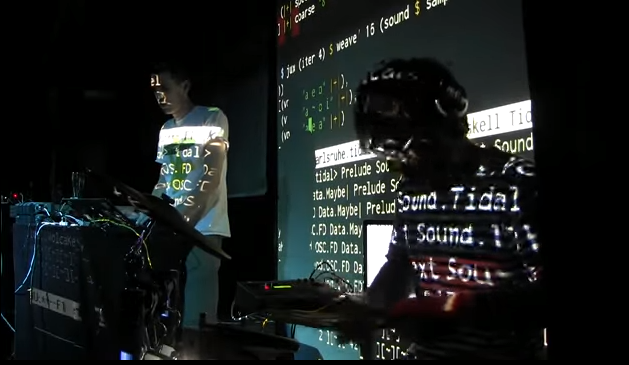
\includegraphics[scale=0.5]{imagens/canute.png}
  \caption{Performance do duo Canute (Karlesruhe, 2015) \textbf{Fonte}: \citeonline{mclean_canute_2015}.}
  \label{fig:canute}
\end{figure}
\end{frame}

% ----------------- NOVO SLIDE --------------------------------
\begin{frame}{Algorave}
\begin{figure}[h]
  \centering
  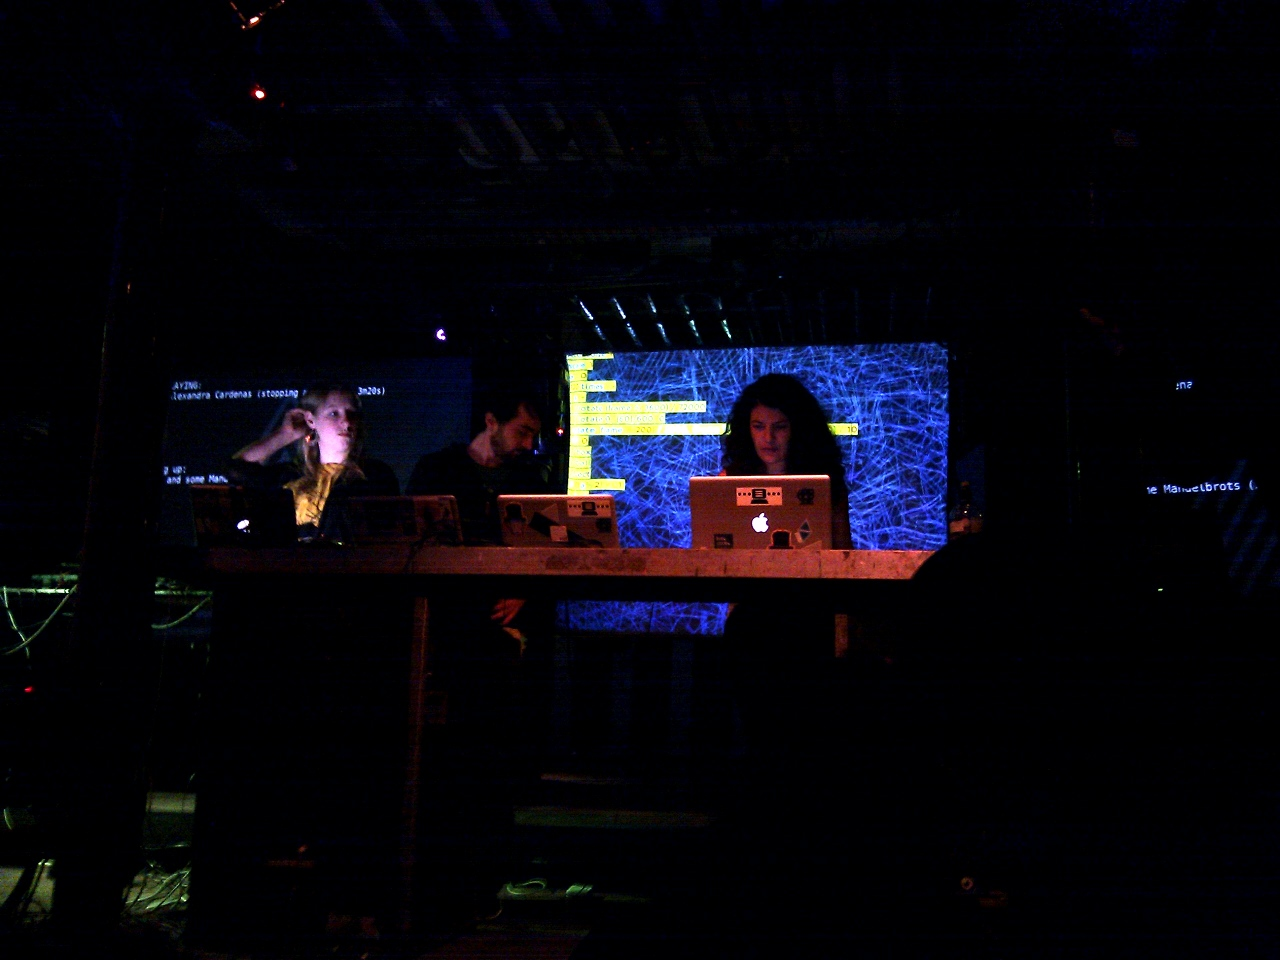
\includegraphics[scale=0.2]{imagens/cardenas.jpg}
  \caption{Performance de Alexandra Cárdenas (Londres, 2013) \textbf{Fonte}: \citeonline{griffths_algorave_2013}.}
  \label{fig:cardenas}
\end{figure}
\end{frame}

% ----------------- NOVO SLIDE --------------------------------
\begin{frame}{Algorave}
\begin{figure}[!h]
  \centering
  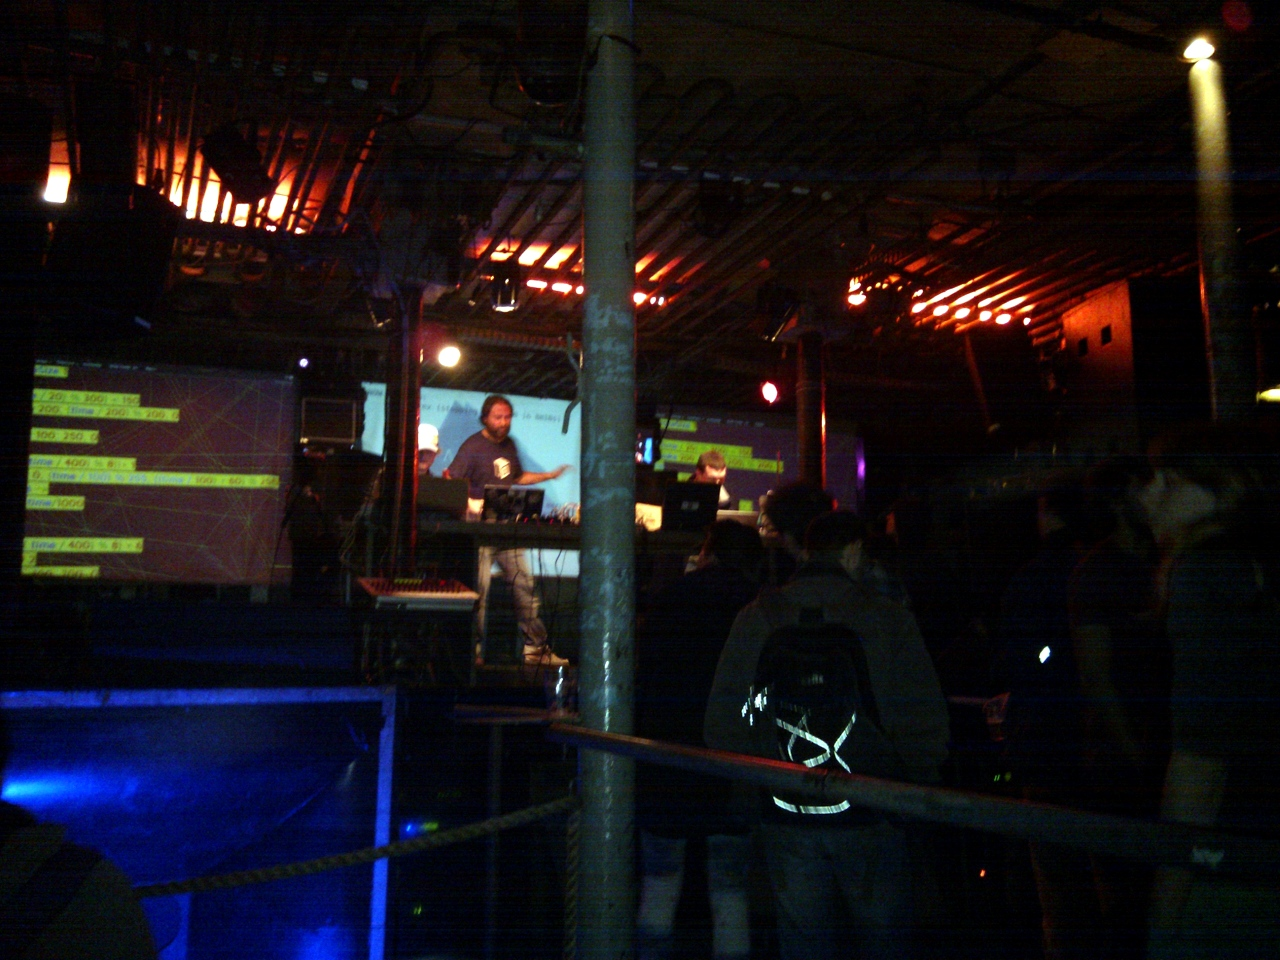
\includegraphics[scale=0.2]{imagens/algorave.jpg}
  \caption{Performance do duo Mico Rex (Londres, 2013) \textbf{Fonte}: \citeonline{griffths_algorave_2013}.}
  \label{fig:micorex}
\end{figure}
\end{frame}

% ----------------- NOVO SLIDE --------------------------------
\begin{frame}{Coreografia}
Kate Sichio

• \emph{Hacking the Body}/\emph{Hacking Choreography};

• \emph{Hacking Coreography} \emph{v.01} e \emph{v.02});

• \emph{Hacking The Body 2.0};
\end{frame}

% ----------------- NOVO SLIDE --------------------------------
\begin{frame}{Coreografia}
Para \citeonline[cap.~1, p.~3]{downie_choreography_2005}, do ponto de vista computacional, a partitura coreográfica é mais próxima do código escrito em uma linguagem de computador do que a partitura musical tradicional. 
\end{frame}

% ----------------- NOVO SLIDE --------------------------------
\begin{frame}{Coreografia}
• Assimilação do pensamento algorítmico na Dança $\rightarrow$ \emph{Sensibilidades Computacionais} \apud[cap.~1, p.~3;p.~31]{downie_choreography_2005}{sichio_hacking_2004} 

• \emph{mecanismos de generalização e abstração, representação da coreografia e dança como computação} \cite[cap.~1, p.~2--4]{downie_choreography_2005} $\rightarrow$ estratégias elaboradas por coreógrafos como Merce Cunningham, Trisha Brown, Bill T. Jones, e William Forsythe.
\end{frame}

% ----------------- NOVO SLIDE --------------------------------
\begin{frame}{Coreografia}
\emph{Esta sensibilidade computacional é presente em dois níveis em um trabalho destes coreógrafos. Primeiramente, em seus processos coreográficos -- os sistemas, métodos, e notação através dos quais os coreógrafos criam a dança. Segundo, no trabalho ele mesmo, finalizado, que aparece no palco e é interpretado pelo observador. As primeiras invenções e proclamoções de Cunningham -- a democracia do espaço do palco, e a redescoberta do que está atrás do dançarino como ponto de origem do movimento -- pode ser interpretado como generalizações do tipo; qualquer ponto do palco é a ``frente'', e conectado por um conjunto de articulações pode ser pensado como um membro. O que eram constantes, uma vez especificados em uma descrição rígida, se tornam variáveis em uma estrutura generativa.}\cite[cap.~1, p.~2--4]{downie_choreography_2005}
\end{frame}

% ----------------- NOVO SLIDE --------------------------------
\begin{frame}{Hacking Coreography}
Duas experiências com uma Partitura de Eventos do artista Alison Knowles (mais especificamente a peça de performance \#8, de 1965)
\end{frame}

% ----------------- NOVO SLIDE --------------------------------
\defverbatim{\oito}{
\scriptsize \begin{verbatim}
Divida uma variedade de objetos em dois grupos. 
Cada grupo é rotulado com "tudo". 
Estes grupos podem incluir diversas pessoas. 
Existe uma terceira divisão do palco, objetos vazios, rotulados com "nada". 
Cada um dos objetos é "alguma coisa". 
Um executante combina e ativa os objetos das seguintes maneiras para qualquer duração 
   desejada de tempo :

* "alguma coisa" com "tudo"

* "alguma coisa" com "nada"

* "alguma coisa" com "alguma coisa"

* "tudo" com "tudo"

* "tudo" com "nada"

* "nada" com "nada"
\end{verbatim}
}

\begin{frame}{Hacking Coreography}
\oito
\end{frame}

\begin{frame}{Hacking Coreography v.01}
\emph{Depois que a partitura foi completada, contudo, ela foi \emph{hackeada}. Isso significa que o executante tenta de alguma forma contornar as instruções originais. Isto foi feito sem preparações prévias e a audiência assistiu isso se desdobrar enquanto era realizada. Nesta primeira performance, o papel e os rótulos foram rasgados para criar novas palavras e categorias (\ldots) Então ao invés de ``nada''$[$Nothing$]$, foram formados dois grupos, ``não''$[$No$]$ e ``coisa''$[$Thing$]$.} \cite[p.~31]{sichio_hacking_2004}
\end{frame}

\begin{frame}{Hacking Coreography v.02}
Orientações são escritas como um híbrido de texto discursivo, legível por um executante, e de código de computador em linguagem Java. Isto é, ele não é executável por um computador para resultar em sons, mas por um humano para resultar em movimentos.
\end{frame}

\begin{frame}{Hacking Coreography v.02}
Orientações são escritas como um híbrido de texto discursivo, legível por um executante, e de código de computador em linguagem Java. Isto é, ele não é executável por um computador para resultar em sons, mas por um humano para resultar em movimentos.
\end{frame}

\defverbatim{\danca}{
\begin{minted}[fontsize=\scriptsize]{java}
/Dance/
set up()
{
dance a centre, right
dance b centre, left
}

movement()
{
move1 (dance a = rotate) (dance b = jump)
move2 (dance a = brush) (dance b = lie down)
move3 (dance a = push) (dance b = run)
move4 (dance a = step) (dance b = kneel)
}

coreography()
{
if (dancer a = rotate right 180)
then both jump = 2 feet to 1
if (dancer b = travels)
then brush = right foot
}

run(){
move1
move4
move4
move1
move2
move3
move1
move2
move3
move4
}

/hack/
{
if (dancer a = kneel)
dancer a = kneel
if (dancer a = rotate)
dancer b = rotate opposite direction 
}
\end{minted}
}

\begin{frame}[allowframebreaks]{Hacking Coreography v.02}
\danca
\end{frame}

\begin{frame}[allowframebreaks]{Hacking The Body}
\emph{Esta peça é uma exploração de eletrônica codificada ao vivo e movimentos improvisados. Uma dançarina veste uma peça de atuadores hápticos. Estes atuadores são programados em tempo-real via OSC\footnote{N.A.: ``\emph{Open Sound Control} é um protocolo de comunicação entre computadores, sintetizadores sonoros e outros dispositivos multimídia que são otimizados para as modernas tecnologias de rede''. Disponível em \url{http://opensoundcontrol.org/introduction-osc}} para 'zunir' sobre os lados direito e esquerdo da dançarina para indicar qual lado do corpo a dançarina deve mover. A partitura é codificada ao vivo pela coreógrafa enquanto a dançarina responde por uma retroalimentação háptica. Esta peça explora o \emph{live coding} de corpos, e movimento como saída, ao invés de saídas sonoras ou visuais como encontrado em muitas execuções de \emph{live coding}
}

\begin{figure}[!h]
  \centering
  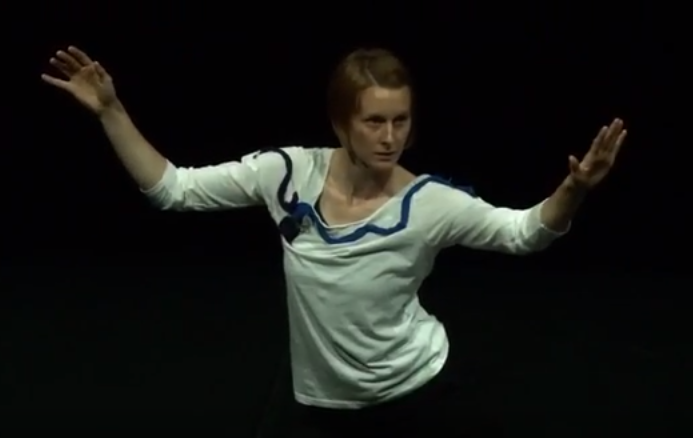
\includegraphics[scale=0.3]{imagens/iclcdanca.png}
  \caption{Dançarina (anônima) controlada por Kate Sicchio (2015) através de uma codificação improvisada. \textbf{Fonte}: \url{https://www.youtube.com/watch?v=uAq4BAbvRS4}.}
  \label{fig:iclcdanca}
\end{figure}
\end{frame}

\begin{frame}{Música computacional}
• FooBarBaz      (Aspecto histórico, em um evento nacional)

• Magno Calliman (Aspecto performático, em um evento nacional)

• Supercopair    (Aspecto telemático, com pesquisadores brasileiros)
\end{frame}

\defverbatim{\chuck}{
\begin{minted}[fontsize=\scriptsize]{c}
["samples/fx/s20.wav"] @=> Foo.name;
[0.] @=> Foo.prop;
[.25, .15] @=> Foo.rate;
[2., 1., 1., 4.] @=> Foo.du;
[.8] @=> Foo.gain;
\end{minted}
}

\begin{frame}[allowframebreaks]{Foo Bar Baz}
FooBarBaz é um grupo de improvisação de códigos formado por Gilson Beck, Renato Fabbri, Ricardo Fabbri e Vilson Vieira. Sua primeira apresentação foi durante o Festival Contato 2011. Os membros são ativos em um laboratório virtual conhecido como \emph{labMacambira}(\url{http://labmacambira.sourceforge.net/}).

\begin{figure}[!h]
  \centering
  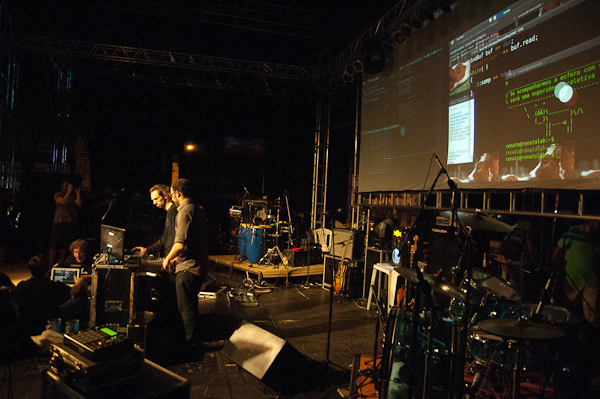
\includegraphics[scale=0.45]{imagens/Foobarbaz1.jpg}
  \caption{Festival Contato, 2011. \textbf{Fonte}: \citeonline{fabbri_wiki_2011}.}
  \label{fig:foobarbaz}
\end{figure}
\end{frame}

\begin{frame}{Foo Bar Baz}
\chuck
\end{frame}


\begin{frame}{Foo Bar Baz}
Funcionamento $\rightarrow$ \emph{grade temporal} (TimeGrid) $\rightarrow$  Graham Coleman (\url{http://www.dtic.upf.edu/~gcoleman/}).
\end{frame}

\defverbatim{\timegrid}{
\begin{minted}[fontsize=\scriptsize]{c}
//basic timing operations abbreviated

public class TimeGrid {

    dur beat;
    dur meas;
    dur sect;

    int nbeat;
    int nmeas;

    //phase and magnitude of offset
    float measPhase;
    dur measOffset;
    ...

    //sync to beat
    fun void sync() {
        beat - (now % beat) => now;
    }

    fun void sync(dur T) {
        T - (now % T) => now;
    }

    //how long to sync to this duration
    fun dur syncDur(dur T) {
	return (T - (now % T));
    }

    //minimum time
    fun dur tmin(dur a, dur b) {
	return (a < b) ? a : b;
    }
    ...
}
\end{minted}
}  

\begin{frame}[allowframebreaks]{Foo Bar Baz}
\timegrid
\end{frame}

\begin{frame}[allowframebreaks]{screenBashing}
Performance de \emph{screenBashing} de Magno Caliman (ver \autoref{fig:screenbashing}), realizada durante o XIII ENCUN\footnote{Encontro Nacional de Compositores Universitários em Campinas-SP no ano de 2015.}. 

\begin{figure}[!h]
  \centering
  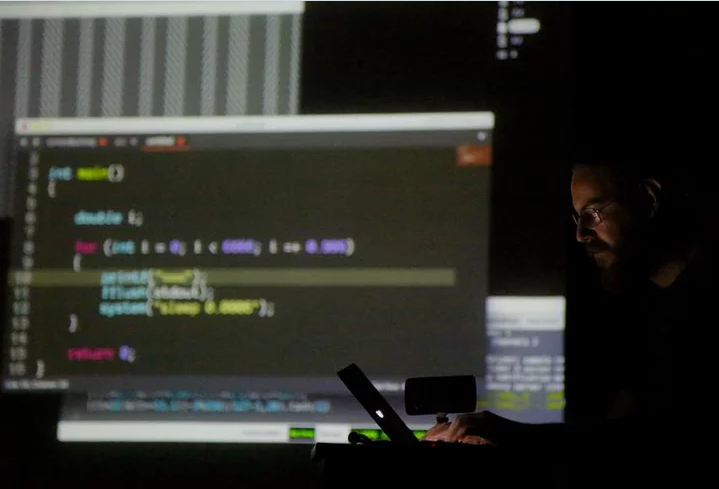
\includegraphics[scale=0.5]{imagens/screenbashing.png}
  \caption{Performance de \emph{screenBashing}. \textbf{Fonte}: \url{https://vimeo.com/148626379}.}
  \label{fig:screenbashing}
\end{figure}
\end{frame}

\begin{frame}{screenBashing}
\emph{Não acho totalmente adequado considerar como puramente um improviso. (\ldots) acredito que se imaginarmos um \emph{continuum}, uma linha onde de um lado vc tem uma improvisação totalmente livre (impossível de se alcançar, claro) e do outro uma composição 100\% determinada (tão impossível quanto), acredito que \emph{screenBashing} está posicionada mais à direita\ldots}
\end{frame}

\defverbatim{\magnoA}{
\begin{minted}[fontsize=\scriptsize]{c}
# include <stdio.h>

int main()
{
  double i;
  
  for (int i=0; i<; i < 6666; i=+0.999)
  {
      printf("\\\\    //  \\");
      fflush(stdout)
      system("sleep 0.0006")
  }
}
\end{minted}
}

\defverbatim{\magnoB}{
\begin{minted}[fontsize=\scriptsize]{bash}
# gcc - compilador
# a.c - arquivo em linguagem c
# -o  - escreve o resultado em um outro arquivo
# a   - arquivo binario alvo
\$> gcc a.c -o a
magno.c: In function 'main':
magno.c:7:12: error: conflicting types for 'i'
\end{minted}
}

\defverbatim{\magnoC}{
\begin{minted}[fontsize=\scriptsize]{bash}
\\\\    //  \\\\\\    //  \\\\\\    //  \\\\\\    //  \\\\\\    //
  \\\\\\    //  \\\\\\    //  \\\\\\    //  \\\\\\    //  \\\\\\  
  //  \\\\\\    //  \\\\\\    //  \\\\\\    //  \\\\\\    //  \\\\
\\    //  \\\\\\    //  \\\\\\    //  \\\\\\    //  \\\\\\    //  
\\\\\\    //  \\\\\\    //  \\\\\\    //  \\\\\\    //  \\\\\\    
//  \\\\\\    //  \\\\\\    //  \\\\\\    //  \\\\\\    //  \\\\\\
    //  \\\\\\    //  \\\\\\    //  \\\\\\    //  \\\\\\    //  \\\
\\\    //  \\\\\\    //  \\\\\\    //  \\\\\\    //  \\\\\\    //  
\\\\\\    //  \\\\\\    //  \\\\\\    //  \\\\\\    //  \\\\\\    /
/  \\\\\\    //  \\\\\\    //  \\\\\\    //  \\\\\\    //  \\\\\\  
  //  \\\\\\    //  \\\\\\    //  \\\\\\    //  \\\\\\    //  \\\\\
\    //  \\\\\\    //  \\\\\\    //  \\\\\\    //  \\\\\\    //  \\
\\\\    //  \\\\\\    //  \\\\\\    //  \\\\\\    //  \\\\\    /
\end{minted}
}  

\begin{frame}[allowframebreaks]{screenBashing}
Código-fonte:

\magnoA

Execução:

\magnoB

Resultado:

\magnoC
\end{frame}

\begin{frame}{screenBashing}
• O código sonoro foi pouco exposto

• Valorização ideológica. $\rightarrow$ repetição dos algarismos seis e nove $\rightarrow$ \emph{black metal} abstrato (?) 

• uma segunda notação (Capítulo 3), mais enxuta e sem erros, permite apontar a questão ideológica
\end{frame}

\defverbatim{\magnoD}{
\begin{minted}[fontsize=\scriptsize]{c}
# include <stdio.h>
int main(){
  int i=0;
  for (;;i++){
      printf("=====  ______");
      fflush(stdout);
      // 30 frames por segundo 
      // ou um limite aproximado da
      // pecepcao humana (1/30)
      system("sleep 0.033");
  }
}
\end{minted}
}  

\defverbatim{\magnoE}{
\begin{minted}[fontsize=\scriptsize]{bash}
=====  ______=====  ______=====  ______=====  ______=====  ______=====
  ______=====  ______=====  ______=====  ______=====  ______=====  ___
___=====  ______=====  ______=====  ______=====  ______=====  ______==
===  ______=====  ______=====  ______=====  ______=====  ______=====  
______=====  ______=====  ______=====  ______=====  ______=====  _____
_=====  ______=====  ______=====  ______=====  ______=====  ______====
=  ______=====  ______=====  ______=====  ______=====  ______=====  __
____=====  ______=====  ______=====  ______=====  ______=====  ______=

\end{minted}
}

\begin{frame}{screenBashing}
Código-fonte:

\magnoD

Resultado:

\magnoE
\end{frame}

\begin{frame}{Telepresença e espaços virtuais}
• Uma rede local, com computadores diferentes, mas com os improvisadores fisicamente próximos;

• Uma rede remota, privada, que comunica um conjunto de pessoas fisicamente distantes \citeonline[p.~152--153]{junior_supercopair_2015}

• O navegador de \emph{internet} se torna o ambiente virtual de criação musical \cite{roberts_web_2013}.
\end{frame}

\begin{frame}{Telepresença e espaços virtuais}
\emph{live coding sessions} $\rightarrow$ sessões de improvisações que ocorrem em encontros, simpósios e \emph{workshops}, ricamente documentadas (\url{https://supercollider.github.io/archive}).
\end{frame}

\begin{frame}{Telepresença e espaços virtuais}
Performance telepresencial em 2014, por Ben Swift, Henry Gardner e Andrew Sorensen, realizada entre dois intérpretes-programadores localizados na Alemanha e Estados Unidos usando um servidor SSH localizado na Australia \cite[p.~152--153]{junior_supercopair_2015}
\end{frame}

\begin{frame}{Telepresença e espaços virtuais}
\emph{Supercopair} (\url{https://github.com/deusanyjunior/atom-supercopair}) $\rightarrow$ ambiente cooperativo de improvisação de códigos.
\end{frame}

\begin{frame}{Telepresença e espaços virtuais}
Execuções remotas em navegadores de \emph{internet}, com auxílio da biblioteca \emph{WebAudio API} (\url{https://dvcs.w3.org/hg/audio/raw-file/tip/webaudio/specification.html}).
\end{frame}

\begin{frame}{Telepresença e espaços virtuais}
• \emph{Gibber} \cite{roberts_gibber:_2012} (\url{http://gibber.mat.ucsb.edu/}); 

• \emph{Wavepot}(\url{http://www.wavepot.com});

• \emph{Vivace} \cite{vieira_vivace:_2015} (\url{http://void.cc/freakcoding})

• \emph{Termpot} \cite{lunhani_termpot_2015} (\url{http://jahpd.github.io/termpot})
\end{frame}

\section{Definições Históricas da Improvisação de códigos}
\begin{frame}{Definições Históricas da Improvisação de códigos}
Exemplos proto-históricos $\rightarrow$ possuem similaridades com o conjunto de regras práticas publicadas por \cite{ward_live_2004}
\end{frame}


\begin{frame}{Definições Históricas da Improvisação de códigos}
• Pietro Grossi
  
• Baía de São Franscisco
\end{frame}

\begin{frame}{Definições Históricas da Improvisação de códigos}
Evento Histórico: Live Algorithm Programming and Temporary Organization for its Promotion
\end{frame}

\begin{frame}{Pietro Grossi -- Computer Concerto}
\emph{Grossi começou a se interessar por música computacional durante a primeira metade doas anos 60, quando ele quando ele organizou um programa de rádio centrado em torno da "música inovadora" em geral \cite{giomi_conversasioni_1999}. Contudo a primeira experiência de Grossi com um computador foi em Milão, no Centro de Pesquisa Elétrica da Olivetti-General. Aqui, auxiliado por alguns técnicos internos e engenheiros, ele conseguiu compor e gravar alguns de seus primeiros trabalhos em música computacional. Eles foram, em sua maior parte, transcrições de música clássica ocidental. Contudo, houve algumas exceções, por exemplo, uma faixa chamada Mixed Paganini} \cite[p.~126]{mori_pietro_2015}
\end{frame}

\begin{frame}{Pietro Grossi -- DCMP (\emph{Digital Computer Music Program})}
\emph{Um dos mais importantes aspectos do trabalho de Grossi foi que todas intervenções eram instantâneas: o operador não tinha que esperar pelo computador terminar todas operações requisitadas, e depois ouvir os resultados. Cálculos de dados e reprodução sonoras eram simultâneos. \textbf{Esta simultaneidade não era comum no campo da \emph{Computer Music} daquele tempo, e Grossi deliberadamente escolheu trabalhar desta forma, perdendo muito no lado da qualidade sonora. Seu desejo era poder escutar os sons resultantes imediatamente}} \cite[p.~126]{mori_pietro_2015}
\end{frame}

\begin{frame}{Pietro Grossi -- DCMP (\emph{Digital Computer Music Program})}
``preguiçoso'' (\emph{pigro}, \emph{lazy}) $\rightarrow$ \emph{reflexividade}
\end{frame}

\begin{frame}{Pietro Grossi -- DCMP (\emph{Digital Computer Music Program})}
\emph{habilidade de um programa manipular como dados algo que representa o estado do programa durante sua própria execução, o mecanismo para codificação de estados de execução é chamado \emph{reificação}}.\cite[p.~1]{malefant_reflection_1996}.
\end{frame}

\begin{frame}{Pietro Grossi -- DCMP (\emph{Digital Computer Music Program})}
\emph{Naquele tempo, os recursos de cálculo eram escassos e, para obter a reprodução em tempo-real citada, era necessário pedir por pouca quantidade de dados. (\ldots) A síntese de timbres necessita de uma quantidade imensa de dados, e então a escolha foi descartá-la temporariamente, e todos os sons eram reproduzidos com o timbre de uma onda quadrada. Esta forma de onda era gerada por extração do estado binário do \emph{pin} de saída da placa mãe que controla o programa. Essa saída tinha um único \emph{bit}, e então a onda sonora gerada era o resultado desta mudança do estado binário. Desta forma, o computador não emprega quaisquer recursos para calcular a síntese sonora, economizando-os para o processo de produção musical. Grossi não estava interessado na qualidade da saída sonora em sua primeira fase em Pisa. O que importava particularmente era a capacidade em trabalhar em tempo real, ou, em outras palavras, para ter a escolha de escutar imediatamente ao que ele escreveu no teclado do terminal de vídeo} \apud{giomi_conversasioni_1999}{mori_pietro_2015}.
\end{frame}

\begin{frame}{Pietro Grossi -- TAU2-TAUMUS (\emph{Terminale Audio 2$^a$ versione)}}
Grossi foi capaz de implementar melhorias de timbre, digitalmente controladas por doze vozes, com síntese analógica.
\end{frame}

\begin{frame}{Pietro Grossi -- TAU2}
\emph{Estas doze vozes eram divididas em três grupos, compostos de quatro canais cada. O operador poderia atribuir um timbre diferente para cada grupo, que era modulado usando síntese aditiva com sete sobretons. Cada sobretom era controlado individualmente pelo programa.}
\end{frame}

\begin{frame}{Pietro Grossi -- TELETAU}
O TAU2-TAUMUS sofreu uma considerável modificação, sendo que era possível controlar o sistema digital-analógico remotamente. O novo programa foi batizado de TELETAU \citeonline[p.~128--129]{mori_pietro_2015}
\end{frame}

\begin{frame}{Pietro Grossi -- TELETAU}
\emph{Grossi fez sua primeira experiência do tipo durante uma conferência de tecnologia em Rimini em 1970, onde o músico reproduzia algumas de suas composições, bem como sons randômicos, empregando um terminal de vídeo conectado pelo telefone para o computador da CNR em Pisa. A RAI, empresa de radiodifusão italiana, emprestou suas pontes de rádio $[$Comunicação entre duas antenas$]$ para enviar sinais sonoros entre Pisa e Rimini. É como se fosse o primeiro experimento de telemática musical no mundo} \cite[p.~129]{mori_pietro_2015}.
\end{frame}

\begin{frame}{Baía de São Franscisco}
• The League of Automatic Composers

• The Hub

• Ron Kuivilla
\end{frame}

\begin{frame}{Baía de São Franscisco}
\emph{Mills College} em Oakland. 
\end{frame}

\begin{frame}{Baía de São Franscisco}
\emph{Com o florescimento da indústria de computadores pessoais na Baía de São Franscisco, o acesso às novas tecnologias e pessoas que desenvolveram elas era talvez o melhor no mundo. (\ldots) Esta também é a cultura que deu ao mundo a música ``New Age'', uma versão aguada e comercializada das músicas com base em modos e drones que Terry Riley, Pauline Oliveros, e LaMonte Young inventaram durante os anos cinquenta e sessenta. Mas a música feita na Costa Oeste também incluiam improvisações barulhentas e livre de restrições, que sobraram das revoluções contra-culturais dos anos 60}\cite{brown_indigenous_2013}.
\end{frame}

\begin{frame}{The League of Automatic Composers}
• Segunda metade da década de setenta: Jim Horton começa a adquirir micro-controladores KIM-1 (\emph{Keyboard Input Monitor}, \url{http://www.6502.org/trainers/buildkim/kim.htm}), com interesses musicais. 

• David Behrman e John Bischoff, Rich Gold, Cathy Morton, Paul Robinson, e Paul Kalbach.
\end{frame}

\begin{frame}{KIM1}
\begin{figure}[!h]
  \centering
  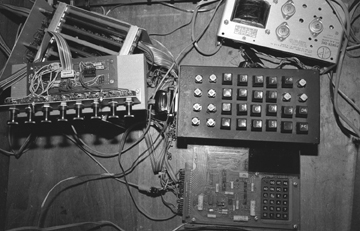
\includegraphics[scale=0.7]{imagens/siskim1.jpg}
  \caption{Sistema de música computacional de John Bischof \emph{circa} 1980. Foto: Eva Shoshanny\protect\footnotemark. \textbf{Fonte}: \citeonline{brown_indigenous_2013}.}
  \label{fig:siskim1}
\end{figure}
\end{frame}

\begin{frame}{The League of Automatic Composers}
Na primavera de 1979, montamos uma série quinzenal regular de apresentações informais sob os auspícios da \emph{Bay Center for the Performing Arts}. Todos outros domingos à tarde passávamos algumas horas configurando nossa rede de KIMs na sala \emph{Finnish Hall}, na Berkeley, e deixávamos a rede tocando, com retoques aqui e ali, por uma ou duas horas. Os membros da audiência poderiam ir e vir como quisessem, fazer perguntas, ou simplesmente sentar e ouvir. Este foi um evento comunitário de tipos como outros compositores aparecendo, tocando ou compartilhando circuitos eletrônicos que tinham projetado e construído. Um interesse na construção de instrumentos eletrônicos de todos os tipos parecia estar "no ar". Os eventos da sala \emph{Finn Hall} foram feitos para uma cena com paisagens sonoras geradas por computador misturado com os sons de grupos de dança folclórica ensaiando no andar de cima e as reuniões ocasionais do Partido Comunista na sala de trás do edifício velho venerável. A série durou cerca de 5 meses que eu me lembre.\cite{brown_indigenous_2013}
\end{frame}

\begin{frame}{The League of Automatic Composers}
• Tim Perkis

• Sam Ashley, Kenneth Atchley, Ben Azarm, Barbara Golden, Jay Cloidt e Brian Reinbolt.
\end{frame}

\begin{frame}{The League of Automatic Composers}
``rede de composições''
\end{frame}

\begin{frame}{The League of Automatic Composers}
\emph{Os membros da liga geralmente adaptavam composições solo para usar dentro da banda. Estes solos eram desenvolvidos independentemente por cada compositor, e eram tipicamente baseados em esquemas de algoritmos de um tipo ou outro. Existiam características de improvisação diferentes para muitas delas, como bem as músicas eram diferentes em detalhes. Teorias matemáticas, sistemas de afinação experimentais, algoritmos de inteligência artificial, projetos de instrumentos de improvisação, e performance interativa eram algumas das áreas exploradas nestes trabalhos (\ldots) Os solos tocavam simultaneamente no cenário de grupo, se tornando ``sub''-composições que interagem, cada uma enviando e recebendo dados pertinentes para o funcionamento musical.}  \cite[12$^o$ parágrafo]{brown_indigenous_2013}.
\end{frame}

\begin{frame}{The Hub}
1986:

• Bischoff e Perkis, após a saída de Horton

• Chris Brown e Mark Trayle

• \emph{THE NETWORK MUSE - Automatic Music Band Festival}. 

• Scott Greham-Lancaster e Richard Zvonar 

• Phil Burk, Larry Polansky e Phil Stone.
\end{frame}

\begin{frame}{The Hub}
• Nome simbólico de um sistema musical centralizado
• \emph{(\ldots) um pequeno microcontrolador como caixa de correio, para postar dados usados no controle de seus sitemas individuais, que eram então acessados por outro intérprete, para usar de qualquer maneira e em qualquer tempo que escolher.}
\end{frame}

\begin{frame}{The Hub}
\emph{\emph{The Hub} originalmente surgiu como uma maneira de limpar uma bagunça. (\ldots) Toda vez que nós ensaiamos, um conjunto complicado de conexões \emph{ad-hoc} entre computadores tinham de ser feitas. Isso criou um sistema com um comportamento rico e variado, mas sujeito a falhas, e trazer outros jogadores ficava difícil. Mais tarde, procuramos uma maneira de abrir o processo, para torná-lo mais fácil para os outros músicos tocarem no contexto de rede. O objetivo era criar uma nova maneira para pessoas fazerem música juntos. A solução bateu no ponto da facilidade de uso, e fornecimento de uma interface de usuário padrão, de modo que os jogadores poderiam conectar praticamente qualquer tipo de computador. \emph{The Hub} é um pequeno computador dedicado a passar mensagens entre os jogadores. Ele serve como uma memória comum, mantendo informações sobre a atividade de cada jogador que seja acessível para os computadores de outros jogadores} \cite[seção 2.1]{brown_indigenous_2013}. 
\end{frame}

\begin{frame}{The Hub}
1987

• Nick Collins e Phil Niblock: curadoria para uma performance telemática entre a \emph{Experimental Media} e \emph{The Clocktower} em Nova York. 

• Divididos em dois trios, se comunicam entre os dois espaços:

  • John Bischoff, Tim Perkis, Mark Trayle;
  
  • Chris Brown, Scot Gresham-Lancaster, e Phil Stone;
  
  • Dois \emph{Hub} intercomunicáveis. 
  
  • Cada \emph{Hub} era um sistema centralizado para cada trio. 
  
  • ``Simple Degradation'';
  
  • ``Borrowing and Stealing'';
  
  • ``Vague Notions'';
  
  •  performance de um \emph{sexteto acusticamente divorciado mas informacionalmente ligado} \cite[seção 2.2]{brown_indigenous_2013}.
\end{frame}

\begin{frame}{Ron Kuivila}
• 1985: performance de \emph{Water Surfaces}, na STEIM (\emph{STudio for Electro-Instrumental Music}), em Amsterdã \citeonline{mclean_patterns_2009};

• 2007: reconstrução da peça ``\emph{TOPLAP001 - A prehistory of live coding}'' ( \url{http://toplap.org/wiki/TOPLAP_CDs}.); 
\end{frame}

\begin{frame}{Water Surfaces}
\emph{Esta obra usou programação FORTH ao vivo; Curtis \citeonline{roads_steim_1986} testemunhou e relatou a performance de Ron Kuivila feita na STEIM em Amsterdã, em 1985; a performance original termina com a quebra do sistema\ldots}
\end{frame}

\begin{frame}{Water Surfaces}
\emph{Ronald Kuivila programou um computador Apple II no palco para cirar sons densos, rodopiantes e métricos, disposto em camadas e dobravam sobre si. Considerando o equipamento usado, os sons eram surpreendentemente grandes em escala. Kuivila teve problemas em controlar a peça devido q problemas sistêmicos. Ele finalmente entrou em dificuldades técnicas e finalizou a performance} \cite[p.~47]
{roads_steim_1986}.
\end{frame}

\begin{frame}{Water Surfaces}
\emph{Eu vi o \emph{software} FORTH de Ron Kuivila quebrar e queimar no palco em Amsterdã em 1985, mas antes disso, não fez uma música muito interessante. A performance consistiu de digitação}\cite{wang_historical_2005}
\end{frame}

\begin{frame}{\emph{Live Algorithm Programming and Temporary Organization for its Promotion}}

• Manifesto elaborado por \citeauthoronline{ward_live_2004,mclean_patterns_2009};

• DJ, Música algorítmica, Música de Processos;

• Regras práticas do \emph{livecoding} publicadas por artistas-programadores ingleses;
\end{frame}

\begin{frame}{LAPTOP}
\emph{O \emph{Livecoding} permite a exploração de espaços algorítmicos abstratos como uma improvisação intelectual. Como uma atividade intelectual, pode ser colaborativa. Codificação e teorização podem ser atos sociais. Se existe um público, revelar, provocar e desafiar eles com uma matemática complexa se faz com a esperança de que sigam, ou até mesmo participem da expedição. Estas questões são, de certa forma, independentes do computador, quando a valorização e exploração do algoritmo é o que importa. Outro experimento mental pode ser encarado com um DJ ao vivo codificando e escrevendo uma lista de instruções para o seu \emph{set} (feito com o iTunes, mas aparelhos reais funcionam igualmente bem). Eles passam ao HDJ $[$ \emph{Headphone Disk Jockey} $]$ de acordo com este conjunto de instruções, mas no meio do caminho modificam a lista. A lista está em um retroprojetor para que o público possa acompanhar a tomada de decisão e tentar obter um melhor acesso ao processo de pensamento do compositor} \cite[p.~245]{ward_live_2004}.
\end{frame}

\begin{frame}{LAPTOP}
• Música como um Processo Gradual\footnote{\cfcite{reich_music_1968}}

• A ligação conceitual do \emph{live coding} com a Música de Processos e a Música Generativa é relativa ao uso de algoritmos  mas não ao resultado sonoro como processo de escuta.

• Música Minimalista de Processos é apresentada por \citeonline[p.~128]{mailman_agency_2013} $\rightarrow$ Música de Algoritmos Simples,  um processo determinístico que age sobre focos de quadros temporais. 

• Música Generativa é sensitiva às circuntâncias, isso quer dizer que irá reagir diferentemente dependendo das suas condições iniciais, onde ocorre e assim por diante.
\end{frame}

\begin{frame}{LAPTOP}
\emph{Na codificação ao vivo a performance é o processo de desenvolvimento de \emph{software}, em vez de seu resultado. O trabalho não é gerado por um programa acabado, mas através de sua jornada de desenvolvimento do nada para um algoritmo complexo, gerando mudanças contínuas da forma musical ou visual ao longo do caminho. Isto contrasta com a arte generativa popularizada pela música geradora de Brian \citeonline{eno_generative_1996}. (\ldots) O resultado segue mais ou menos o mesmo estilo, com apenas algumas permutações, dando uma idéia das qualidades da peça. Isto é bem ilustrado pelo nosso estudo de caso de um artista-programador, que executa seu programa poucas vezes não para produzir novas obras, mas para obter diferentes perspectivas sobre o mesmo trabalho.}
\end{frame}


\begin{frame}[allowframebreaks]{TOPLAP}
Permutação na ordem das letras do acrônimo LAPTOP dá origem ao acrônimo TOPLAP. \citeonline[p.~246]{ward_live_2004} e \citeonline{ramsay_algorithms_2010} apontam que este acrônimo dinâmico; isto quer dizer que as primeira, terceira  e quinta letras possuem diversos significados

\begin{figure}[!h]
  \centering
  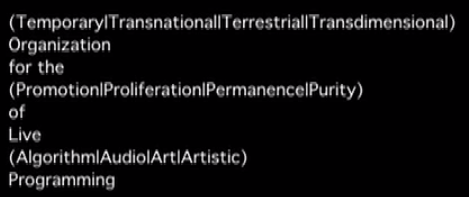
\includegraphics[scale=0.6]{imagens/TOPLAP.png}
  \caption{Definição do siginificado de TOPLAP. \textbf{Fonte}: \citeonline{ramsay_algorithms_2010}.}
  \label{fig:TOPLAP}
\end{figure}

\emph{A organização TOPLAP (www.toplap.org), cuja sigla possui diversas interpretações, uma sendo \emph{Organização Temporária para a Proliferação da Programação de Algoritmos Ao Vivo}, foi criada para promover e explorar o \emph{live coding}. TOPLAP nasceu em um bar enfumaçada em Hamburgo à uma da manhã em 15 de Fevereiro de 2004} \cite[p.~246]{ward_live_2004}.

\end{frame}

\begin{frame}{Manifesto Lubeck04}

Escrito em um ônibus, é maisconhecido como ``\emph{Show us your screens}'', e prescreve algumas regras práticas do \emph{live coding} \cite[p.~247]{ward_live_2004}. 
\end{frame}

\begin{frame}[allowframebreaks]{Manifesto Lubeck04}
Exigimos:

• Acesso à mente do intérprete, para todo o instrumento humano.

• Obscurantismo é perigoso. Mostre-nos suas telas.

• Programas são instrumentos que podem modificar eles mesmos.

• O programa será transcendido - Língua Artificial é o caminho.

• O código deve ser visto assim como ouvido, códigos subjacentes visualizados bem como seu resultado visual.

• Codificação ao vivo não é sobre ferramentas. Algoritmos são pensamentos. Motosserras são ferramentas. É por isso que às vezes algoritmos são mais difíceis de perceber do que motosserras.

Reconhecemos contínuos de interação e profundidade, mas preferimos:

• Introspecção dos algoritmos.

• A externalização hábil de algoritmo como exibição expressiva/impressiva de destreza mental.

• Sem \emph{backup} (minidisc, DVD, safety net computer).

Nós reconhecemos que:

• Não é necessário para uma audiência leiga compreender o código para apreciar, tal como não é necessário saber como tocar guitarra para apreciar uma performance de guitarra.

• Codificação ao vivo pode ser acompanhada por uma impressionante exibição de destreza manual e a glorificação da interface de digitação.

• Performance envolve contínuos de interação, cobrindo talvez o âmbito dos controles, no que diz respeito ao parâmetro espaço da obra de arte, ou conteúdo gestual, particularmente direcionado para o detalhe expressivo. Enquanto desvios na tradicional taxa de reflexos táteis da expressividade, na música instrumental, não são aproximadas no código, por que repetir o passado? Sem dúvida, a escrita de código e expressão do pensamento irá desenvolver suas próprias nuances e costumes. 
\end{frame}

\begin{frame}{Manifesto Lubeck04}
• ``Obscurantismo é perigoso. Mostre-nos suas telas''

• ``Algoritmos são pensamentos, motosserras são ferramentas''
\end{frame}

\begin{frame}{Mostre-nos suas telas}
• ``\emph{Using Contemporary Technology in Live Performance; the Dilemma of the Performer}'' \cite{schloss_dilemma_2003}

• Crítica ao sétimo dos questionamentos sugeridos para uma performance de improvisação ao vivo com computadores \citeauthoronline{ward_live_2004}.
\end{frame}

\begin{frame}[allowframebreaks]{Mostre-nos suas telas}
1. Causa-e-efeito é importante, pelo menos para o observador/audiência em uma sala de concerto. 
\ \\
2.Corolário: Mágica na performance é bom. Muita mágica é fatal! (chato).
\ \\
3. Um componente visual é essencial para a audiência, tal como existe um aparato visual de entrada para parâmetros e gestos.
\ \\
4. Sutileza é importante. Grandes gestos são facilmente visíveis de longe, o que é bom, mas eles são movimentos de desenho animado se comparados à execução de um instrumento musical.
\ \\
5. Esforço é importante. Neste sentido, nós estamos em desvantagem de desempenho na performance musical com o computador.
\ \\
6. Improvisação no palco é bom, mas ``mimar'' o aparato no palco não é improvisação, é edição. É provavelmente mais apropriado fazer isso no estúdio antes do concerto, ou se durante o concerto, com o console no meio ou atrás da sala de concerto.
\ \\
7. Pessoas que representam devem representar. Um concerto de música de computador não é uma desculpa/oportunidade para um programador(a) se sentar no palco. Sua presença melhora ou impede o desempenho da representação?
\end{frame}

\begin{frame}{Algorithms are Thoughts, Chainsaws are Tools}
Vídeo de Stephen \citeonline{ramsay_algorithms_2010}, publicado no Vimeo, em  27 de fevereiro de 2010, como um \emph{Coffee-Table Movie}. É uma análise pessoal da performance de \emph{Strange Places} de Andrew Sorensen.
\end{frame}

\begin{frame}{Algorithms are Thoughts, Chainsaws are Tools}
Algoritmo como pensamento é um espaço conceitual abstrato
\end{frame}

\begin{frame}{Algorithms are Thoughts, Chainsaws are Tools}
\emph{A noção de partitura não se aplica aqui, é como não fosse possível aplicá-lo ao músico de \emph{jazz} ou tocador de \emph{bluegrass}. (\ldots). Levanta a questão, para mim, se, em uma sessão de \emph{livecoding} *feita*, constite simplismente no ato de digitar em um programa existente, seria tão convincente -- eu acho que isso pode definitivamente ter pontos de interesse. Ou qual seria o análogo do \emph{livecoding} para uma performance não-improvisada de música?}
\end{frame}

\begin{frame}{Algorithms are Thoughts, Chainsaws are Tools}
\emph{O que torna o \emph{livecoding} diferente, e pode a performance de música tradicional imitar isso? Para responder esta questão, parece importante notar que as formas nas quais a música improvisada muitas vezes apela para alguma noção de autenticidade ou gênio. Enquanto o \emph{livecoding} ele mesmo à noção de virtuosismo de código, ``autenticidade'' parece fora de lugar aqui. Se música improvisada sugere expressão, o \emph{livecoding} sugere um conjunto de restrições na expressão, descrevendo os parâmetros através dos quais a máquina $[$midi$]$ ganha expressão}
\end{frame}

\section{Metodologia de análise de uma Improvisação musical de códigos}
\begin{frame}{Metodologia de análise de uma Improvisação musical de códigos}
• Taxonomia de tipos de criatividade $\rightarrow$ o \emph{Quadro Conceitual de Sistemas Criativos}(\emph{Creative System Frameworks}, ou CSF);

• Discretização (amostragem) de processos criativos contínuos;

• Modelo de estruturação, e análise, de improvisações de códigos musicais.
 capítulo.
 \end{frame}
 
 
\begin{frame}{Criatividade}
• Criatividade \cite{boden_creative_1990};

• Criatividade, códigos e imagens mentais \cite{McLean2011}

• Comportamento Criativo por Bricolagem;

• Quadro Conceitual de sistemas criativos

• O modelo de improvisação
\end{frame}

\begin{frame}{Paradoxo da Criatividade}
• Paradoxo da Criatividade: ``Capacidade que o falante de uma língua tem de criar novos enunciados sem que os tenha ouvido ou dito anteriormente.'' (\url{http://www.priberam.pt/dlpo/criatividade});
\end{frame}

\begin{frame}{Paradoxo Criatividade}
\emph{O ponto inicial de Boden para o desenvolvimento de sua explicação, é a observação de que o conceito de criatividade contém um paradoxo. Por definição, criatividade cria, i.e., produz alguma coisa nova. Mas se estamos comprometidos com uma abordagem mecanicista do mundo -- nenhum milagre é permitido -- iremos acreditar que tudo o que ocorre é, em princípio, previsível. Iremos acreditar também que qualquer coisa nova deve ser construída de componentes existentes. Isso implica que nada pode ser intrinsicamente novo.}\cite[p.~2]{thornton_quantitative_2007}
\end{frame}

\begin{frame}{Paradoxo da Criatividade}
Valorização de distinções $\rightarrow$ \emph{Para justificar a classificação de uma idéia criativa... alguém deve identificar os princípios generativos com respeito ao que é impossível} \apud[p.~51;~p.~3]{boden_creative_1990}{thornton_quantitative_2007}
\end{frame}

\begin{frame}{Taxonomia da Criatividade}
\emph{A distinção é entre o sentido de criar um conceito que nunca foi criado antes $[$criatividade-P$]$, e um conceito que nunca foi criado antes por um criador específico $[$criatividade-H$]$. (\ldots) no trabalho de Boden, existe uma distinção entre criatividade exploradora e transformacional, que será relevante aqui, e então merece alguma explicação. \textbf{Boden concebe o processo de criatividade como uma identificação e/ou localização de novos objetos conceituais em um espaço conceitual}.}
\end{frame}

\begin{frame}{Taxonomia da Criatividade}
\begin{figure}
\centering
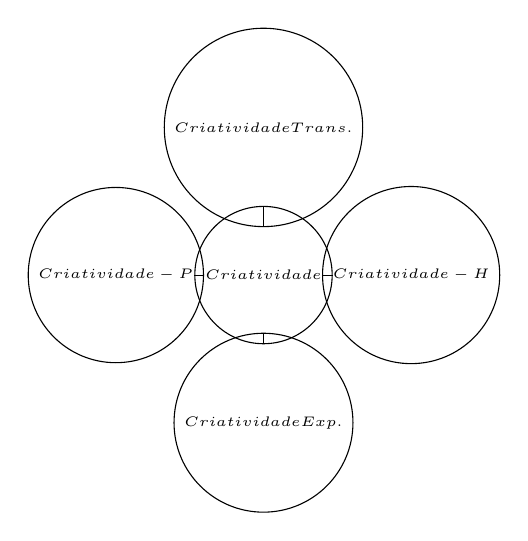
\begin{tikzpicture}[scale=2.5]
\tikzstyle{every node}=[draw,shape=circle];
\path (0:0cm) node (v0) {\tiny $Criatividade$};
\path (0:0.75cm) node (v1) {\tiny $Criatividade-H$};
\path (2*90:0.75cm) node (v2) {\tiny $Criatividade-P$};
\path (3*90:0.75cm) node (v3) {\tiny $Criatividade Exp.$};
\path (90:0.75cm) node (v4) {\tiny $Criatividade Trans.$};
\draw (v0) -- (v1)
(v0) -- (v2)
(v0) -- (v3)
(v0) -- (v4);
\end{tikzpicture}
\caption{Classificação da criatividade : 1) criatividade-psicológica/criatividade-histórica; 2) critividade exploradora/criatividade transformacional. \textbf{Fonte}: autor com base em \citeonline{wiggins_framework_2006}.}
\label{fig:ortogonal}
\end{figure}
\end{frame}

\begin{frame}{Taxonomia da Criatividade}
\emph{De fato, na primeira edição $[$1990$]$, ela não oferece uma explicação do número de diferentes tipos de criatividade que ela identificou. Parece que sua intenção era distinguir os dois tipos notados, espaços conceituais devem ter uma característica generativa. E isso certamente é a interpretação comum. Ainda no sumário 'em uma casca de noz' de sua teoria, foi adicionado um prólogo à segunda edição \cite{boden_creative_1990}, e em \citeonline{boden_creativity_1998}, ela coloca que sua explicação distingue três principais formas de criatividade, sendo exploração, transformação e \emph{combinação}. É somada à incerteza a observação que somente a definição forte $[$generalizadora$]$ da definição possui o poder de resolver o paradoxo da criatividade}
\end{frame}

\begin{frame}{Taxonomia da Criatividade}
• \emph{comportamento combinatorial}, imagens poéticas, analogias -- onde duas idéias novas associadas compartilham heranças de estruturas conceituais --, piadas \cite[p.~348]{boden_creativity_1998}

• \emph{comportamento explorador} de algo $\rightarrow$ de espaços conceituais estruturados;

• \emph{comportamento transformacional} $\rightarrow$ a exploração resulta em estruturas ("idéias") que não são novidades, mas inesperadas. Considerado por Boden como a ``criatividade genuína''.
\end{frame}

\begin{frame}{Taxonomia da Criatividade}
• Wiggins $\rightarrow$ classificação exploradora/transformacional ao enunciar quatro axiomas dos Sistemas Criativos \citeonline[p.~3--4]{thornton_quantitative_2007} 

• Utilização de heurísticas e mapas para identificar conceitos valiosos dentre de um espaço conceitual existente (exploração guiada). 
\end{frame}

\begin{frame}{Definição de Criatividade}
Axiomas abrem espaço para uma definição generalizadora:

\begin{table}[!h]
\caption{Definições formais de criatividade por \citeonline[p.~451]{wiggins_framework_2006}}
\small
    \begin{tabular}{ | p{4cm} | p{7.25cm} |}
    \hline 
    \hline 

    \tiny{Criatividade} 
    & \tiny{``O estudo e suporte, através de meios e métodos computacionais, do comportamento exibido por sistemas naturais e artificiais, que podem ser considerados criativos se exibidos em humanos.'' } \\
    \hline

    \tiny{Computação criativa} 
    & \tiny{``O estudo e suporte, através de meios e métodos computacionais, do comportamento exibido por sistemas naturais e artificiais, que são considerados criativos''. } \\
    \hline

    \tiny{Sistemas criativos} 
    & \tiny{``Uma coleção de processos, naturais ou automáticos, que são capazes de alcançarem ou simularem comportamentos que em humanos seriam considerados criativos''} \\
    \hline

    \tiny{Comportamento Criativo} 
    & \tiny{``Um ou mais dos comportamentos exibidos por um sistema criativo''} \\
    \hline
    \hline
   
    \end{tabular}
\label{tab:criatividade}
\end{table}
\end{frame}

\begin{frame}{Criatividade, códigos e imagens mentais}
• Comportamento criativo como o processo de estruturação uma \emph{imagem mental}.

• Imagem mental é um símbolo, e seu significado é governado por regras gramaticais e sociais (códigos). 

• Hierarquia de códigos simbólicos, visuais e gramaticais -- Teoria da Codificação Dual \apud[p.~25--29]{paivio_dual_1990}{McLean2011}:
\end{frame}

\begin{frame}{Teoria da Codificação Dual}
\emph{Seu $[$Paivio$]$ argumento não é que existem dois códigos, mas sim que existe uma hierarquia de códigos, que se ramificam no topo em códigos lingüísticos discretos e códigos de percepção contínua, que Paivio nomeia como \emph {logogens} e \emph{imagens} respectivamente. Esta divisão é apresentada em seus processos simultâneos; os seres humanos são capazes de compreender a linguagem ao mesmo tempo que podem ver imagens. (\ldots), é fácil para seres humanos ler um texto enquanto simultaneamente e ouve um discurso. \textbf{A explicação oferecida pela teoria da Codificação Dual é que existem sistemas de símbolos distindos, mas integrados, para linguagens e figuras}.}
\end{frame}

\begin{frame}{Teoria da Codificação Dual}
Para McLean, a teoria da Codificação Dual é suportada pela Neuropsicologia, onde \emph{De maneira muito ampla, o hemisfério esquerdo é especializado para linguagem, e o direito para tarefas visuais-espaciais.}\apud[p.~128--129]{martin2006}{McLean2011}, o que por outro lado, é admitido como uma perigosa generalização. Para exemplificar a formação de imagens (conceitos, lembranças, sentidos) durante a leitura e escrita de texto, apresentaremos um pequeno exemplo de código que formaliza, em uma linguagem de progamação, um simples algoritmo musical.
\end{frame}

\begin{frame}{Teoria da Codificação Dual e Dimensões cognitivas da Notação para linguagens de programação.}

• Tabela auxiliar, usada para fins de criação de linguagens, para a verificação de dimensões cognitivas acessadas durante a atividade de programação.

• As dimensões cognitivas das linguagens visuais são usadas para separar os materiais (o que é representado como material sonoro), da maneira como serão manipulados (o como é representado o material sonoro), durante um fluxo temporal.
\end{frame}

\begin{frame}[allowframebreaks]{Dimensões cognitivas da Notação para linguagens de programação.}
\begin{table}[!h]
\caption{Dimensões cognitivas da Notação para linguagens de programação. \textbf{Fonte}: \apud{church_cognitive_2008}{McLean2011}.}
\small
    \begin{tabular}{ | p{5cm}| p{5cm} |}
    \hline 
    \hline 

    \tiny \textbf{Dimensão} & \textbf{Significado} \\
    \hline 
    \hline 

    \tiny \textbf{Abstração}  
    & \tiny Disponibilidade de mecanismos de abstração \\
    \hline

    \tiny \textbf{Dependências escondidas}

    & \tiny Invisibilidade de ligações importantes entre entidades.\\
    \hline
    
    \tiny \textbf{Compromisso prematuro}  
    & \tiny Restrição na ordem de execução das coisas. \\
  \hline

    \tiny \textbf{Notação secundária}  
    & \tiny Notação diversa da sintaxe formal. \\
    \hline

    \tiny \textbf{Viscosidade}  
    & \tiny Resistência à mudança. \\
    \hline

    \tiny \textbf{Proximidade de mapeamento}  
    & \tiny Proximidade de representação para o domínio-alvo. \\
    \hline

    \tiny \textbf{Consistência}  
    & \tiny Semânticas similares são expressadas em formas sintáticas similares. \\
    \hline
    \hline
    \end{tabular}
\label{tab:dimensoes}
\end{table} 
\ \\
\ \\
\begin{table}[!h]
\small
\begin{tabular}{ | p{5cm}| p{5cm} |}
    \hline 
    \hline 
    \tiny \textbf{Dispersividade}  
    & \tiny Prolixidade da linguagem. \\
    \hline
    
    \tiny \textbf{Tendência ao erro}  
    & \tiny Probabilidade de erros. \\
    \hline

    \tiny \textbf{Operações mentais difíceis}  
    & \tiny Demanda de recursos cognitivos. \\
    \hline

    \tiny \textbf{Provisoriedade}  
    & \tiny Grau de compromisso com ações e marcos. \\
    \hline
    
    \tiny \textbf{Função de expressividade}  
    & \tiny medida em que o efeito de um componente pode ser inferida.\\
    \hline
    \hline
   
    \end{tabular}
\label{tab:dimensoes}
\end{table} 
\end{frame}

\begin{frame}{Comportamento criativo por bricolagem}
No começo o programador tem um conceito meio-formado que só atinge consistência interna através do processo de ser expresso como um algoritmo. O laço interno é onde o programador elabora o objetivo de suas imaginações, e o laço externo é onde essa trajetória está fundamentada na pragmática do que elas realmente têm que fazer. Através deste processo ambos algoritmos e conceitos são desenvolvidos até que o programador sinta que um se aplica com o outro, ou de outra forma julga o processo criativo finalizado.
\end{frame}

\begin{frame}{Comportamento criativo por bricolagem}
\begin{figure}[h]
  \centering
  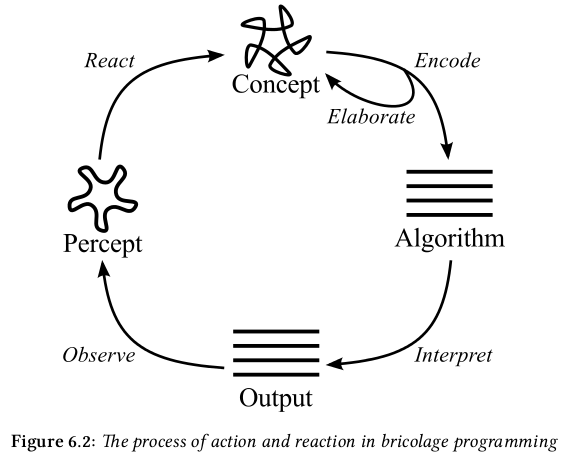
\includegraphics[scale=0.35]{imagens/processo_criativo.png}
  \caption{Modelo de bricolagem para o processo criativo realizado por um artista-programador. \textbf{Fonte}: \citeonline[p.~122]{McLean2011}. }
  \label{fig:processo_criativo}
\end{figure}
\end{frame}

\begin{frame}{Comportamento criativo por bricolagem}
Exemplo de um processo durante a elaboração de uma \emph{estratégia transversal}
\end{frame}

\begin{frame}{Comportamento criativo por bricolagem}
• Imagem mental: um \emph{loop} sincopado, mas bastante regular, descrito em um compasso. Em uma ``partitura-mental'', estruturamos o primeiro tempo com um baixo, que volta a tocar na segunda semicolcheia do terceiro tempo. No Segundo tempo, silêncio. No quarto tempo uma caixa aberta.
\end{frame}

\begin{frame}{Comportamento criativo por bricolagem}
{%
\parindent 0pt
\noindent
\ifx\preLilyPondExample \undefined
\else
  \expandafter\preLilyPondExample
\fi
\def\lilypondbook{}%

\includegraphics{53/lily-86c766d2-1}%
% eof

\ifx\postLilyPondExample \undefined
\else
  \expandafter\postLilyPondExample
\fi
}
\end{frame}

\defverbatim{\haskellA}{
\begin{minted}{haskell}
-- Eletronic Dance Music, BPM = 120 
-- tempo 1 - baixo            (bass)
-- tempo 2 - silencio         (silence)
-- tempo 3 - silencio + baixo
-- tempo 4 - caixa            (sn e sn:4)
d1 \$ (sound "bass3 silence [silence bass3] sn:4")
\end{minted}
}

\begin{frame}[allowframebreaks]{Comportamento criativo por bricolagem}
\haskellA
\end{frame}

\begin{frame}{Comportamento criativo por bricolagem}
{%
\parindent 0pt
\noindent
\ifx\preLilyPondExample \undefined
\else
  \expandafter\preLilyPondExample
\fi
\def\lilypondbook{}%

\includegraphics{c7/lily-46fd6313-1}%
% eof

\ifx\postLilyPondExample \undefined
\else
  \expandafter\postLilyPondExample
\fi
}
\end{frame}

\defverbatim{\haskellB}{
\begin{minted}{haskell}
-- Eletronic Dance Music, BPM = 120 
-- tempo 1 - baixo            (bass)
-- tempo 2 - silencio         (silence)
-- tempo 3 - silencio + baixo
-- tempo 4 - caixa            (sn e sn:4)
d1 \$ (sound "bass3 silence [silence bass3] sn:4")
\end{minted}
}

\begin{frame}{Comportamento criativo por bricolagem}
\haskellB
\end{frame}

\begin{frame}{Comportamento criativo por bricolagem}
{%
\parindent 0pt
\noindent
\ifx\preLilyPondExample \undefined
\else
  \expandafter\preLilyPondExample
\fi
\def\lilypondbook{}%

\includegraphics{2b/lily-de0a8ae3-1}%
% eof

\ifx\postLilyPondExample \undefined
\else
  \expandafter\postLilyPondExample
\fi
}
\end{frame}

\defverbatim{\haskellC}{
\begin{minted}{haskell}
-- Eletronic Dance Music, BPM = 120
-- com uma caixa seca no segundo tempo
-- e uma caixa aberta no quarto tempo
-- A cada 4 tempos, o ritmo diminui pela metade 
-- e depois volta ao normal.
d1 \$ every 4 (density 0.5) (sound "bass3 sn [silence house] sn:4")
\end{minted}
}

\begin{frame}{Comportamento criativo por bricolagem}
\haskellC
\end{frame}

\begin{frame}{Comportamento criativo por bricolagem}
• Para \citeonline[p.~130]{McLean2011},programar ``no momento'', a partir de um arquivo de texto em branco, com uma imagem mental do resultado sonoro (ou visual), caracteriza o processo criativo por bricolagem

\end{frame}

\begin{frame}{Quadro Conceitual de sistemas criativos}
O universo, $\mathcal{U}$, é um espaço multidimensional, no qual dimensões são capazes de representar qualquer coisa, e todos os possíveis conceitos distintos correspondentes àqueles pontos em $\mathcal{U}$ (\ldots) Para tornar a proposta um espaço-tipo possível, permitirei que $\mathcal{U}$ contenha todos os conceitos abstratos, bem como os concretos, e que é possível representar os artefatos tanto completos e incompletos \cite[p.~451]{wiggins_framework_2006}
\end{frame}

\begin{frame}{Quadro Conceitual de sistemas criativos}
Espaços conceituais $\mathcal{C}$, finitos ou infinitos são definidos como restrições de um universo $\mathcal{U}$, caracterizando um conjunto não-determinístico de conhecimentos, representações, e conceitos
\end{frame}

\begin{frame}{Quadro Conceitual de sistemas criativos: axiomas}
\citeonline[p.~452]{wiggins_framework_2006}

• $\mathcal{U}$: um espaço multidimensional, cujas dimensões são capazes de representar qualquer coisa, e todos possíveis conceitos distintos correspondentes com distintos pontos em $\mathcal{U}$.
\end{frame}

\begin{frame}{Quadro Conceitual de sistemas criativos: axiomas}
• Universalidade:  $\mathcal{U}$ pode conter tanto conceitos bem definidos (completos), parcialmente definidos (incompletos), e  o mais incompleto dos conceitos. Os dois primeiros são representados pela letra $c$, enquanto o último é representado por \small{T}. 

• Não-identidade dos conceitos: dois conceitos em  $\mathcal{U}$ são mutuamente diferentes entre si ($c_1 \neq c_2$), e não são um Universo. Esta correção restringe a recursividade de conceitos, o que daria ênfase ao comportamento explorador e anularia a importância do comportamento transformacional.
\end{frame}

\begin{frame}{Quadro Conceitual de sistemas criativos: axiomas}
• Inclusão Universal 1: \emph{espaços conceituais} $\mathcal{C}$ são subconjuntos não-estritos do conunto $\mathcal{U}$. 

• Inclusão Universal 2: conceito vazio, \small{T}, em qualquer espaços conceitual $\mathcal{C}$.
\end{frame}

\begin{frame}{Quadro Conceitual de sistemas criativos}
$\mathcal{U}_{livecoding} = [\mathcal{C}_{Tecelagem}, \mathcal{C}_{Audiovisual}, \mathcal{C}_{Dança}, \mathcal{C}_{Música}, \ldots, \small{T}]$
\end{frame}

\begin{frame}{Quadro Conceitual de sistemas criativos}
\begin{table}[!h]
\caption{Definições formais do Universo de possibilidades de \citeonline{wiggins_framework_2006}, ou Universo de Conceitos por \citeonline{mclean_music_2006}.}
\small
    \begin{tabular}{ | p{3.25cm} | p{4.25cm} | p{4.25cm} |}
    \hline 
    \hline 

    Representação
    & \tiny{Nome}     
    & \tiny{Significado} \\
    \hline

    $c$
    & \tiny{Conceito} 
    & \tiny{Uma instância de um conceito, abstrato ou concreto \cite{wiggins_framework_2006}}. \\
    \hline

    $\mathcal{U}$
    & \tiny{Universo de Conceitos} 
    & \tiny{Superconjunto não restrito de conceitos. \cite{wiggins_framework_2006}. ``Um universo de todos conceitos possíveis'' \cite{mclean_music_2006} }\\
    \hline

    $\mathcal{L}$
    & \tiny{Linguagem} 
    & \tiny{Linguagem utilizada para expressar regras.} \\
    \hline

    $\mathcal{A}$
    & \tiny{Alfabeto} 
    & \tiny{Alfabeto da linguagen que contêm caracteres apropriadospara expressão das regras} \\
    \hline

    $\mathcal{R}$
    & \tiny{Regras de validação} 
    & \tiny{Validam os conceitos em um universo, se apropriados ou não para o espaço trabalhado.} \\
    \hline
    \hline
   
    \end{tabular}
\label{tab:universodeconceitos}
\end{table}
\end{frame}

\begin{frame}{Quadro Conceitual de sistemas criativos}  
\begin{table}[!h]
\caption{Definições formais do Universo de possibilidades de \citeonline{wiggins_framework_2006}, ou Universo de Conceitos por \citeonline{mclean_music_2006}.}
\small
    \begin{tabular}{ | p{3.25cm} | p{4.25cm} | p{4.25cm} |}
    \hline 
    \hline 

    $[[.]]$
    & \tiny{Função de interpretação} 
    & \tiny{``Uma função parcial de $\mathcal{L}$ para funções que resultam em números reais entre [0, 1] (\ldots) 0.5 $[$ou maior$]$ significa uma verdade booleana e menos que 0.5 siginifica uma falsidade booleana; a necessidade disso para valores reais se tornará clara abaixo. }\\
    \hline

     $[[\mathcal{R}]]$
    & \tiny{Regras de validação} 
    & \tiny{Uma função que interpreta $\mathcal{R}$, resultando em uma função indicando aderência ao conceito em $\mathcal{R}$} \\
    \hline

     $\mathcal{C} = [[\mathcal{R}]](\mathcal{U}) $
    & \tiny{Espaço Conceitual} 
    & \tiny{Todos espaços conceituais são um subconjunto não-estrito de $\mathcal{U}$. Um subconjunto contido em $\mathcal{U}$. Uma função que interpreta $\mathcal{R}$, resultando em uma função que indica aderência ao conceito em $\mathcal{R}$. } \\
    \hline

    $\mathcal{T}$
    & \tiny{Regras de detecção} 
    & \tiny{Regras definidas dentro de $\mathcal{L}$ para definir estratégias transversais para localizar conceitos dentro de $\mathcal{U}$.} \\
    \hline
    \hline
   
    \end{tabular}
\label{tab:universodeconceitos}
\end{table}
\end{frame}

\begin{frame}{Quadro Conceitual de sistemas criativos}  
\begin{table}[!h]
\caption{Definições formais do Universo de possibilidades de \citeonline{wiggins_framework_2006}, ou Universo de Conceitos por \citeonline{mclean_music_2006}.}
\small
    \begin{tabular}{ | p{3.25cm} | p{4.25cm} | p{4.25cm} |}
    \hline 
    \hline 

    $\mathcal{E}$
    & \tiny{Regras de qualidade} 
    & \tiny{Conjunto de regras que permitem-nos avaliar qualquer conceito que nós encontramos em $\mathcal{C}$ e determinar sua qualidade, de acordo com critérios que nós considerarmos apropriados. Regras definidas dentro de $\mathcal{L}$ para avaliar a qualidade ou a desejabilidade do conceito $c$.}\\
    \hline

    $<<<\mathcal{R}, \mathcal{T}, \mathcal{E}>>>$
    & \tiny{Função de interpretação} 
    & \tiny{Uma regra necessária para definir o espaço conceitual, ``independentemente da ordem, mas também, ficcionalmente, enumerá-los em uma ordem particular, sob o controle de $\mathcal{T}$ -- isto é cricial para a simulação de um comportamento criativo de um $\mathcal{T}$ particular \cite{wiggins_framework_2006}. Uma função que interpreta a estratégia transversal $\mathcal{T}$, informada por $\mathcal{R}$ e $\mathcal{E}$ . Opera sobre um subconjunto ordenado de $mathcal{U}$ (do qual tem acesso randômico) e resulta em outro subconjunto ordenado de $\mathcal{U}$.'} \\
    \hline
    \hline
   
    \end{tabular}
\label{tab:universodeconceitos}
\end{table}
\end{frame}

\begin{frame}{O modelo de improvisação}
\emph{um esboço para uma teoria geral da improvisação integrada com preceitos da Psicologia Cognitiva (\ldots) teoria do comportamento de improvisação na música} \cite[p.~2]{pressing_improvisation_1987}.
\end{frame}

\begin{frame}{O modelo de improvisação}
• Improvisação particionada em diferentes sequências pode ser parcialmente mapeada em categorias, como blocos sonoros, referentes conceituais e normas estilísticas, conjuntos de objetivos e processos. 
\end{frame}

\begin{frame}{O modelo de improvisação}
\begin{table}[!h]
\caption{Definições formais do Modelo de improvisação de Jeff \citeonline{pressing_improvisation_1987}, segundo \citeonline[p.~2]{mclean_music_2006}.}
\small
    \begin{tabular}{ | p{3cm} | p{5cm} |}
    \hline 
    \hline 

    \tiny{Representação}   
    & \tiny{Significado} \\
    \hline

    $E'$
    & \tiny{Um bloco de eventos sonoros} \\
    \hline

    $K'$
    & \tiny{Uma seqüência de blocos de eventos E, onde um bloco de eventos não se sobrepõe com o seguinte}\\
    \hline

    $I'$
    & \tiny{Uma improvisação, particionada por interrupções em um número de K sequências} \\
    \hline

    $R'$
    & \tiny{Um referente opcional, tal como uma partitura ou uma norma estilística} \\
    \hline
    \hline
   
    \end{tabular}
\label{tab:modelo_improvisacao}
\end{table}
\end{frame}

\begin{frame}{O modelo de improvisação}
\begin{table}[!h]
\caption{Definições formais do Modelo de improvisação de Jeff \citeonline{pressing_improvisation_1987}, segundo \citeonline[p.~2]{mclean_music_2006}.}
\small
    \begin{tabular}{ | p{3cm} | p{5cm} |}
    \hline 
    \hline 
    $G'$
    & \tiny{Um conjunto de objetivos} \\
    \hline

    $M'$
    & \tiny{Uma memória de longo prazo} \\
    \hline

    $O'$
    & \tiny{Um conjunto de objetos} \\
    \hline

    $F'$
    & \tiny{Um conjunto de características dos objetos} \\
    \hline

    $P'$
    & \tiny{Um conjunto de processos} \\
    \hline
    \hline
   
    \end{tabular}
\label{tab:modelo_improvisacao}
\end{table}
\end{frame}

\newcommand{\csf}[2]{
$\mathcal{#1}_{\emph{#2}}$
}


\begin{frame}{Formalização}
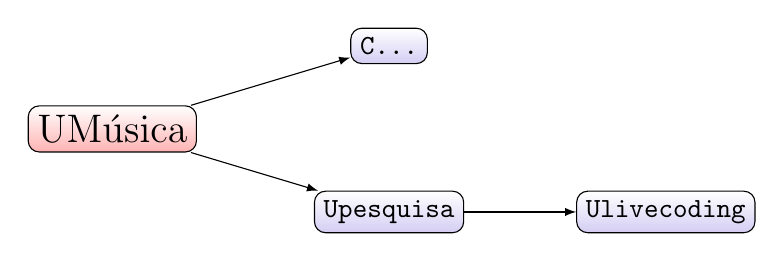
\begin{tikzpicture}
  [
    grow                    = right,
    sibling distance        = 6em,
    level distance          = 10em,
    edge from parent/.style = {draw, -latex},
    every node/.style       = {font=\footnotesize},
    sloped
  ]
  \node [root] {\csf{U}{M\'usica}}
    child { node [env] {\csf{U}{pesquisa}}
      child { node [env] {\csf{U}{livecoding}}}
    }
    child { node [env] {\csf{C}{\ldots}}};
\end{tikzpicture}
\end{frame}

\begin{frame}{Formalização}
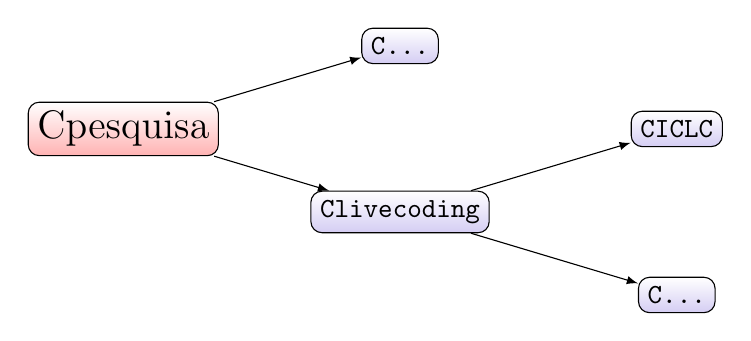
\begin{tikzpicture}
  [
    grow                    = right,
    sibling distance        = 6em,
    level distance          = 10em,
    edge from parent/.style = {draw, -latex},
    every node/.style       = {font=\footnotesize},
    sloped
  ]
  \node [root] {\csf{C}{pesquisa}}
    child { node [env] {\csf{C}{livecoding}}
      child { node [env] {\csf{C}{\ldots}}}
      child { node [env] {\csf{C}{ICLC}}}
    }
    child { node [env] {\csf{C}{\ldots}}}; 
\end{tikzpicture}
\end{frame}

\begin{frame}{Formalização}
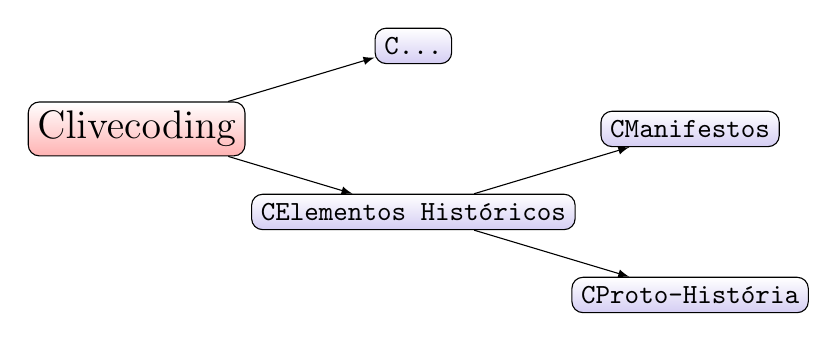
\begin{tikzpicture}
  [
    grow                    = right,
    sibling distance        = 6em,
    level distance          = 10em,
    edge from parent/.style = {draw, -latex},
    every node/.style       = {font=\footnotesize},
    sloped
  ]
  \node [root] {\csf{C}{livecoding}}
    child { node [env] {\csf{C}{Elementos Históricos}}
      child {node [env] {\csf{C}{Proto-História}}}
      child {node [env] {\csf{C}{Manifestos}}}
    }
    child { node [env] {\csf{C}{\ldots}}};
\end{tikzpicture}
\end{frame}

\begin{frame}{Formalização}
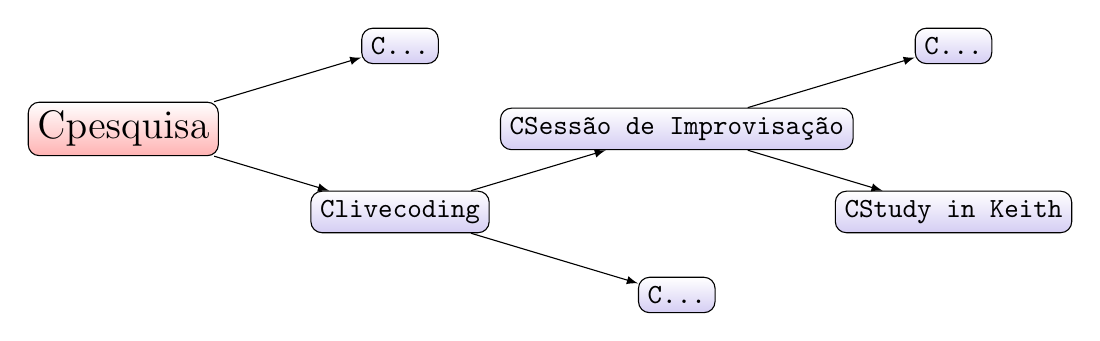
\begin{tikzpicture}
  [
    grow                    = right,
    sibling distance        = 6em,
    level distance          = 10em,
    edge from parent/.style = {draw, -latex},
    every node/.style       = {font=\footnotesize},
    sloped
  ]
  \node [root] {\csf{C}{pesquisa}}
    child { node [env] {\csf{C}{livecoding}}
      child { node [env] {\csf{C}{\ldots}}}
      child { node [env] {\csf{C}{Sessão de Improvisação}}
        child { node [env] {\csf{C}{Study in Keith}}}
        child { node [env] {\csf{C}{\ldots}}}
      }
    }
    child { node [env] {\csf{C}{\ldots}}}; 
\end{tikzpicture}
\end{frame}

\begin{frame}{Formalização}
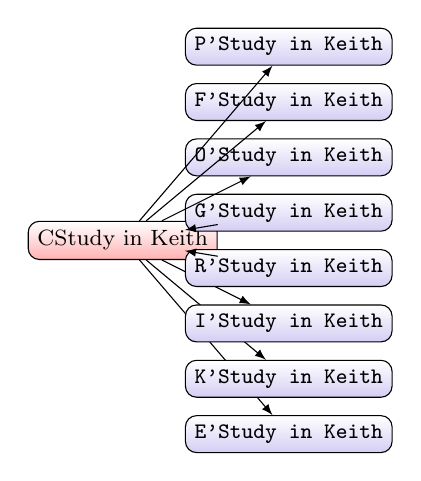
\begin{tikzpicture}
  [
    grow                    = right,
    sibling distance        = 2em,
    level distance          = 6em,
    edge from parent/.style = {draw, -latex},
    every node/.style       = {font=\footnotesize},
    sloped
  ]
  \node [root] {\footnotesize \csf{C}{Study in Keith}}
    child { node [env] {\footnotesize \csf{E'}{Study in Keith}}}
    child { node [env] {\footnotesize \csf{K'}{Study in Keith}}}
    child { node [env] {\footnotesize \csf{I'}{Study in Keith}}}
    child { node [env] {\footnotesize \csf{R'}{Study in Keith}}}
    child { node [env] {\footnotesize \csf{G'}{Study in Keith}}}
    child { node [env] {\footnotesize \csf{O'}{Study in Keith}}}
    child { node [env] {\footnotesize \csf{F'}{Study in Keith}}}
    child { node [env] {\footnotesize \csf{P'}{Study in Keith}}}; 

\end{tikzpicture}
\end{frame}

\newcommand{\pressingthree}[3]{$\mathcal{#1}'^{#3}_{#2}$} 

\begin{frame}{Formalização}
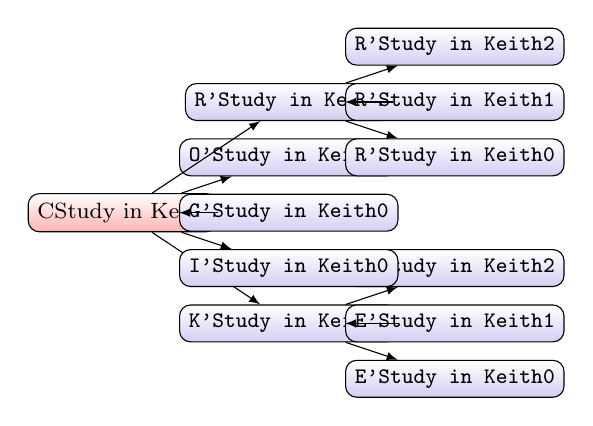
\begin{tikzpicture}
  [
    grow                    = right,
    sibling distance        = 2em,
    level distance          = 6em,
    edge from parent/.style = {draw, -latex},
    every node/.style       = {font=\footnotesize},
    sloped
  ]
  \node [root] {\footnotesize \csf{C}{Study in Keith}}
    child { node [env] {\footnotesize \pressingthree{K'}{Study in Keith}{0}}
      child { node [env] {\footnotesize \pressingthree{E'}{Study in Keith}{0}}}
      child { node [env] {\footnotesize \pressingthree{E'}{Study in Keith}{1}}}
      child { node [env] {\footnotesize \pressingthree{E'}{Study in Keith}{2}}}
    }
    child { node [env] {\footnotesize \pressingthree{I'}{Study in Keith}{0}}}
    child { node [env] {\footnotesize \pressingthree{G'}{Study in Keith}{0}}}
    child { node [env] {\footnotesize \pressingthree{O'}{Study in Keith}{0}}}
    child { node [env] {\footnotesize \csf{R'}{Study in Keith}}
      child { node [env] {\footnotesize \pressingthree{R'}{Study in Keith}{0}}}
      child { node [env] {\footnotesize \pressingthree{R'}{Study in Keith}{1}}}
      child { node [env] {\footnotesize \pressingthree{R'}{Study in Keith}{2}}}
    };

\end{tikzpicture}
\end{frame}

\section{Estudo de caso}
\begin{frame}{Estudo de caso}
\emph{Para fundamentar a discussão em música, considere uma peça de \emph{jazz}, onde \emph{jazz} é um conceito e uma composição particular é uma instância de um conceito. O musicista, explorando os limites do \emph{jazz}, encontra então uma peça para além das regras usuais do \emph{jazz}. Através deste processo, os limites do gênero musical podem ser redefinidos em algum grau, ou se a peça está em um novo terreno particularmente fértil, um novo sub-gênero de \emph{jazz} emerge. Contudo uma peça de música que não quebra limites, de alguma forma pode ser considerada não-criativa \cite[p.~117]{McLean2011}.}
\end{frame}

\begin{frame}{Estudo de caso}
\emph{A Study in Keith} é uma performance de programação ao vivo por Andrew Sorensen, inspirado nos concertos \emph{Sun Bear} de Keith Jarret. Toda a música que você ouve é gerada a partir do código do programa que é escrito e manipulado em \emph{tempo-real} durante a performance. O trabalho foi executado usando o ambiente de desenvolvimento $[$em linguagem$]$ Scheme $[$chamado$]$ Impromptu (\url{http://impŕomptu.moso.com.au}). Não é Keith, mas inspirado por Keith \cite{sorensen_youtube_2014}.
\end{frame}

\begin{frame}{Estudo de caso}
\emph{A Study In Keith} é um trabalho para piano solo (NI's Akoustik Piano), inspirado nos concertos \emph{Sun Bear} de Keith Jarrett. \textbf{Note que não existe som para os dois primeiros 2 minutos da performance, enquanto estruturas iniciais são construídas}. Não é bem Keith, mas inspirado por Keith \cite{sorensen_keith_2009}
\end{frame}

\begin{frame}{Estudo de caso}
Observação e análise de um comportamento criativo musical, de um improvisador-programador, que escreve uma programação-partitura, e realiza a manutenção de um pensamento musical tradicional. Mais especificamente, analisamos o contexto musical de uma simples sequência de blocos sonoros \pressingthree{K}{ask}{0}, gerada por uma função de interpretação $<<<$\csf{R}{ask}, \csf{T}{ask},\csf{E}{ask}$>>>$, cujo referente opcional direto, \pressingthree{R}{ask}{0}, são os Concertos \emph{Sun Bear} de Keith Jarret.
\end{frame}


% ----------------- NOVO SLIDE --------------------------------
\section*{Referências}

% --- O comando \allowframebreaks ---
% Se o conteúdo não se encaixa em um quadro, a opção allowframebreaks instrui 
% beamer para quebrá-lo automaticamente entre dois ou mais quadros,
% mantendo o frametitle do primeiro quadro (dado como argumento) e acrescentando 
% um número romano ou algo parecido na continuação.

\begin{frame}[allowframebreaks]{Referências}
\bibliography{main}
\end{frame}

% ----------------- FIM DO DOCUMENTO -----------------------------------------
\end{document}
